    \documentclass[a4paper,12pt, twoside]{article}
    \usepackage[a4paper, left=2.5cm, right=2.5cm, top=2.5cm, bottom=2.5cm, bindingoffset=0.5cm]{geometry}
    \usepackage[utf8x]{inputenc}
    \usepackage{polski}
    \usepackage[polish]{babel}
    \usepackage{graphicx}
    \usepackage{indentfirst}
    \usepackage{float}
    \usepackage{caption}
    \usepackage{adjustbox}
    \usepackage{array}
    \usepackage{makecell}
    \usepackage{amsmath}
    \usepackage{enumitem}
    \usepackage{afterpage}
    \usepackage{subfig}
    \usepackage{hyperref}
    \usepackage{url}
    \usepackage{listings}
    \usepackage{xcolor}
    %New colors defined below
    \definecolor{codegreen}{rgb}{0,0.6,0}
    \definecolor{codegray}{rgb}{0.5,0.5,0.5}
    \definecolor{codepurple}{rgb}{0.58,0,0.82}
    \definecolor{backcolour}{rgb}{0.95,0.95,0.92}
    
    %Code listing style named "mystyle"
    \lstdefinestyle{mystyle}{
      backgroundcolor=\color{backcolour},
      commentstyle=\color{codegreen},
      keywordstyle=\color{magenta},
      numberstyle=\tiny\color{codegray},
      stringstyle=\color{codepurple},
      basicstyle=\ttfamily\footnotesize,
      breakatwhitespace=false,         
      breaklines=true,                 
      captionpos=b,                    
      keepspaces=true,                 
      numbers=left,                    
      numbersep=5pt,                  
      showspaces=false,                
      showstringspaces=false,
      showtabs=false,                  
      tabsize=2
    }
    
    \lstset{style=mystyle}
    
    
    \renewcommand\thesection{\arabic{section}.}
    \renewcommand\thesubsection{\arabic{section}.\arabic{subsection}.}
    \renewcommand\thesubsubsection{\arabic{section}.\arabic{subsection}.\arabic{subsubsection}.}
    \renewcommand{\lstlistingname}{Algorytm}% Listing -> Algorytm
    \frenchspacing
    \setlength{\parindent}{.5cm}
    \makeatletter
    \setlength{\@fptop}{0pt}
    \makeatother
    \linespread{1.5}
    \begin{document}
    	\newpage
    	\thispagestyle{empty}
    	\begin{center}
    		
    		\begin{figure}
    			\centering
    			
\includegraphics[width=7cm]{images/polsl_logo.jpg}
    			\vspace{.5cm}
    		\end{figure}
    		
    		{\fontsize{17}{17}\selectfont
    			\textsc{Politechnika Śląska \\[.3cm]
    				Wydział Automatyki, Elektroniki i Informatyki  \\[.3cm]
    				Kierunek Teleinformatyka  \\[1.5cm]}
    			\textbf{Projekt inżynierski \\[0.7cm]}}
    		
    		\Large
    		{Elektroniczna plakietka konfigurowana z urządzenia mobilnego \\[3.5cm]}
    		\Large{\begin{flushleft}
    				Autor: Jakub Legutko\\
    				Kierujący pracą: dr inż. Grzegorz Dziwoki\\[0.3cm]
    		\end{flushleft}}
    		
    		\normalsize
    		\vfill Gliwice, styczeń 2020
    	\end{center}
    	\newpage
    	\leavevmode\thispagestyle{empty}\newpage
    	\newpage
    	\thispagestyle{empty}
    	\tableofcontents
    	\newpage
    	\leavevmode\thispagestyle{empty}\newpage
    	\newpage
    	\clearpage
    	\setcounter{page}{1}
    	
    	\section{Wstęp}
    	
    	\subsection{Wprowadzenie}
    	Zmiany klimatyczne są coraz bardziej widoczne na świecie. Wycinka drzew jest jednym z głównych powodów wzrostu emisji gazów cieplarnianych\cite{clima_causes}, ograniczenie jej wpłynie pozytywnie na poziom dwutlenku węgla w atmosferze, co przełoży się na polepszenie klimatu. 
    	
    	Druk wizytówek oraz identyfikatorów pochłania znaczące ilości papieru, jak również tuszu w skali globalnej ze względu na ich jednorazowe wykorzystanie w większości przypadków. Z tego powodu ważne jest znalezienie alternatywnej metody. Gdyby zamiast papieru wykorzystać urządzenie, z którego można korzystać wielokrotnie poprzez zmianę wyświetlanych danych, zmniejszylibyśmy zapotrzebowanie na papier, zmniejszając jednocześnie emisję dwutlenku węgla. Oprócz papieru potrzebnego do wytworzenia plakietek nie będziemy również marnować toneru, którego produkcja pochłania około 3.2 kilograma gazów cieplarnianych\cite{cartidge_production} na kartridż zawierający 200 gramów toneru. Kolejną rzeczą jest recykling, któremu trzeba poddać niepotrzebne już identyfikatory oraz zużyte do ich produkcji kartridże.
    	
    	Idealnym rozwiązaniem takiego problemu wydaje się papier elektroniczny (ang. \textit{e-paper}). Wyświetlane na nim dane można modyfikować dowolną ilość razy, dzięki czemu może być wykorzystywany wielokrotnie, nie powodując zużycia dodatkowych surowców po każdym wyprodukowaniu nowym użyciu. Po wyświetleniu dostarczonych danych wyświetlacz nie pobiera żadnej energii, dzięki takiemu rozwiązaniu może być używany bez dodatkowych baterii lub innych alternatywnych źródeł dostarczanej energii.
    	
    % 	\newpage
    	
    	
    	\subsection{Cel projektu}
    	Celem projektu inżynierskiego jest zaprojektowanie elektronicznej plakietki identyfikującej, mogącej zastąpić identyfikatory lub wizytówki z wykorzystaniem wyświetlacza typu e-papier. Prezentowane dane są przygotowywane i przesyłane przy pomocy urządzenia mobilnego za pomocą napisanej aplikacji.
    
    	\subsection{Założenia projektowe}
    	Przed przystąpieniem do wykonania projektu przyjęto podane niżej założenia projektowe:
    	\begin{itemize}
    		\item użycie wyświetlacza wykonanego w technologii papieru elektronicznego
    		\item mobilność działania plakietki 
    		\item łączność bezprzewodowa pomiędzy ekranem a urządzeniem wysyłającym dane
    		\item aplikacja na system Android
    		\item przechowywanie w aplikacji wpisów z danymi do wyświetlania
    		\item wyświetlanie danych w różnych miejscach na ekranie 
    		\item przechowywanie układów wyświetlania danych w pamięci urządzenia
    	\end{itemize}
    % 	\newpage
    	
    	\subsection{Opis projektu}
    	Do realizacji projektu wykonano prototyp urządzenia, składający się z mikrokontrolera oraz ekranu w technologii papieru elektronicznego. Dla urządzenia przesyłającego dane wykonano aplikację mobilną, posiadającą funkcję wysyłania oraz przechowywania danych. 
    	
    	Wybór jednostki sterującej wybrano głównie dla prostoty i krótkiego czasu wykonania prototypu. Jedną z ważniejszych rzeczy, którą powinien posiadać mikrokontroler była wbudowana technologia łączności bezprzewodowej  jaką są np. \textit{Bluetooth}\cite{bluetooth} lub \textit{Wi-Fi}\cite{wifi}. 
    	
    	Ostatecznie zdecydowano o wykorzystaniu w projekcie protokołu \textit{Bluetooth} do bezprzewodowej transmisji danych z urządzenia mobilnego do mikrokontrolera. Głównym powodem dla wyboru \textit{Bluetootha} jest występowanie tej technologii w zdecydowanej większości urządzeń mobilnych dostępnych na rynku, dzięki czemu wykonany projekt będzie mógł być użyty przez szeroką gamę urządzeń.
    	
    	\begin{flushleft}
    	Wykonanie projektu przebiegło w kilku etapach:
    	\begin{itemize}
    	    \item wykonanie prototypu urządzenia
    	    \item napisanie programu sterującego mikrokontrolerem
    	    \item napisanie aplikacji dla urządzenia mobilnego
    	    \item przeprowadzenie testów urządzeń i aplikacji
    	\end{itemize}
    	\end{flushleft}
    	
    % 	\newpage
    	\section{Realizacja projektu}
    	Do wykonania projektu użyto następujących technologii oraz narzędzi. Wykorzystane przy projektowaniu i programowaniu narzędzia są udostępniane w ramach licencji zezwalających na korzystanie z nich bez opłat w projektach komercyjnych.
    	
    	\subsection{Narzędzia programistyczne}
    	\subsubsection{Android Studio}
    	Android Studio jest oficjalnym zintegrowanym środowiskiem programistycznym \textit{(ang. integrated development environment)}\cite{ide} do produkcji aplikacji na system Android, bazowanym na IntelliJ IDEA.
    	
    	\begin{figure}[H]
    	    \centering
    		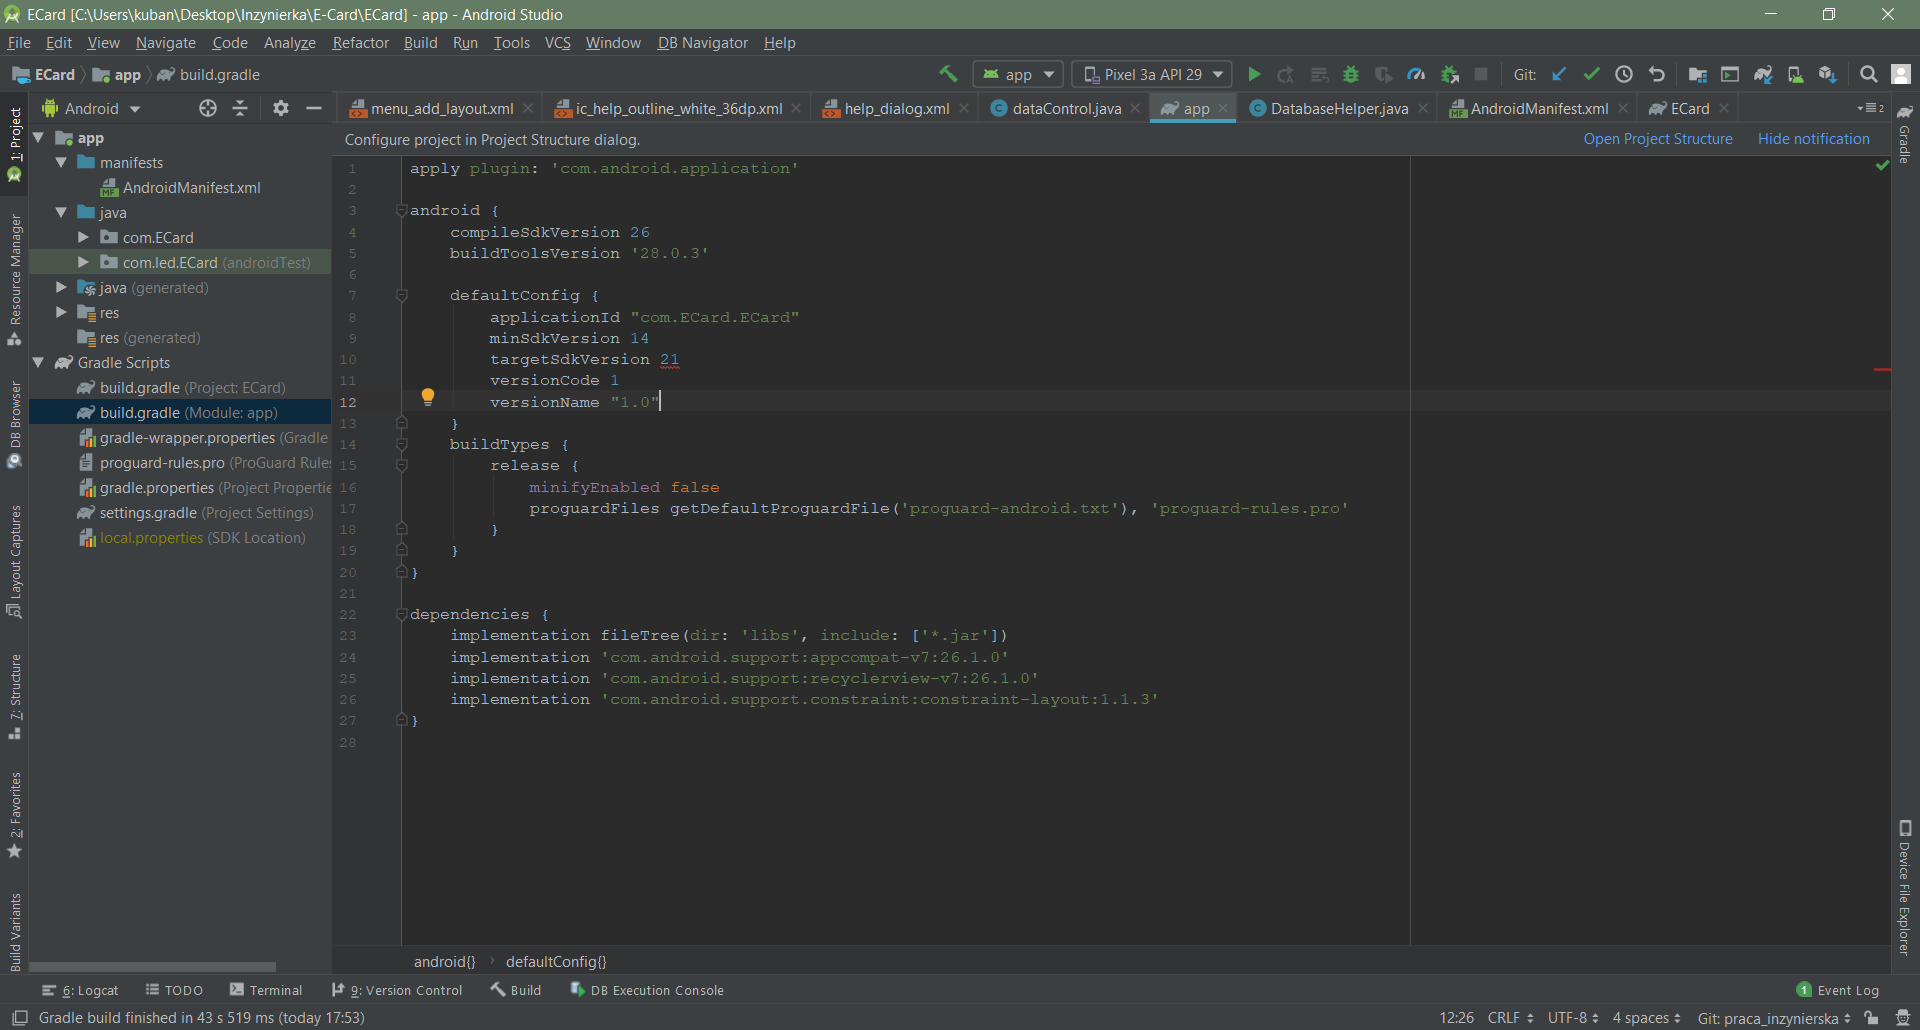
\includegraphics[width=1\textwidth]{images/rys4_android.png}
    		\caption{Widok Android Studio}
            \label{fig:androidstudio}
    	\end{figure}
    	
    	\begin{flushleft}
    	Oprócz posiadanie czołowych możliwości edycji kodu i wbudowanych zaawansowanych narzędzi programistycznych cechuje się również:
    	\begin{itemize}
    	    \item elastycznym narzędziem służącym do budowania projektów opartym na Gradle\cite{gradle}
    	    \item szybkim i bogatym w funkcje emulatorem, mogącym zastąpić do testowania większość urządzeń dostępnych z systemem Android
    	    \item zunifikowanym środowiskiem do produkcji aplikacji na wszystkie urządzenia z systemem Android
    	    \item szablonami kodu i integracją z GitHub
    	    \item obszernymi narzędziami do testowania kodu i aplikacji
    	    \item narzędziami do wykrywania błędów składni \textit{Lint}\cite{lint}, niezgodności wersji i innych błędów
    	    \item wsparciem \textit{Native Development Kit}\cite{ndk}
    	\end{itemize}
    	\end{flushleft}
    	
    	\subsubsection{Git}
    	Git jest to rozproszony system kontroli wersji stworzony przez Linusa Torvaldsa. Jest wolnym oprogramowaniem opublikowanym na licencji GNU GPL v2.0, z pierwszą wersją wydaną w roku 2005.
    	
    	Git śledzi wszelkie różnice dokonane w plikach, pozwala wrócić do dowolnej wcześniejszej wersji. Daje możliwość podglądu wszystkich zmian, które były wykonane w pliku z dokładnością do zmian wykonanych w każdej linii kodu. Jest przystosowany do pracy w zespołach składających się z wielu osób. Każda osoba będąca w projekcie ma możliwość zobaczenia zmian wprowadzanych przez inne osoby.
    	
    	Jedną z najbardziej przydatnych funkcji Gita, jest system zarządzania gałęziami. Dzięki niemu wiele osób może pracować nad różnymi funkcjonalnościami aplikacji jednocześnie. Bez przeszkadzania sobie. Następnie możliwe jest proste i szybkie dołączanie wykonanych zmian do głównej gałęzi projektu.
    	
    		\begin{figure}[H]
    			\centering
    			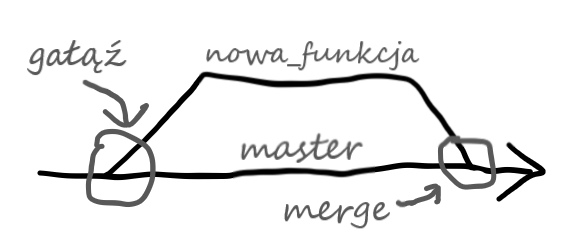
\includegraphics[width=8cm]{images/rys1_branches.png}
    			\caption{Schemat wykorzystania gałęzi}
                \label{fig:branching}
    		\end{figure}
    
    	Uzyskujemy dzięki temu większą kontrolę nad projektem, która przekłada się na mniejszą ilość błędów i większą ilość czasu, którą można przeznaczyć na tworzenie nowych funkcjonalności niż na ręczne składanie kodu w wiele osób.\cite{git}
    	
    	\subsubsection{GitKraken}
    	GitKraken jest graficznym klientem Gita dostępnym na wiele platform. Zbudowany został przez AxoSoft w 2014 roku. GitKraken upraszcza używanie skomplikowanych komend tekstowych wiersza poleceń\cite{cli} wykorzystywanego do obsługi Git. Pozwala na korzystanie ze zdalnych repozytoriów poprzez integrację z takimi systemami jak np. GitHub, GitLab czy Bitbucket. W aplikacji wbudowane są narzędzia rozwiązywania konfliktów scalania, dostępny jest również edytor tekstowy.
    	\begin{figure}[H]
    	    \centering
    		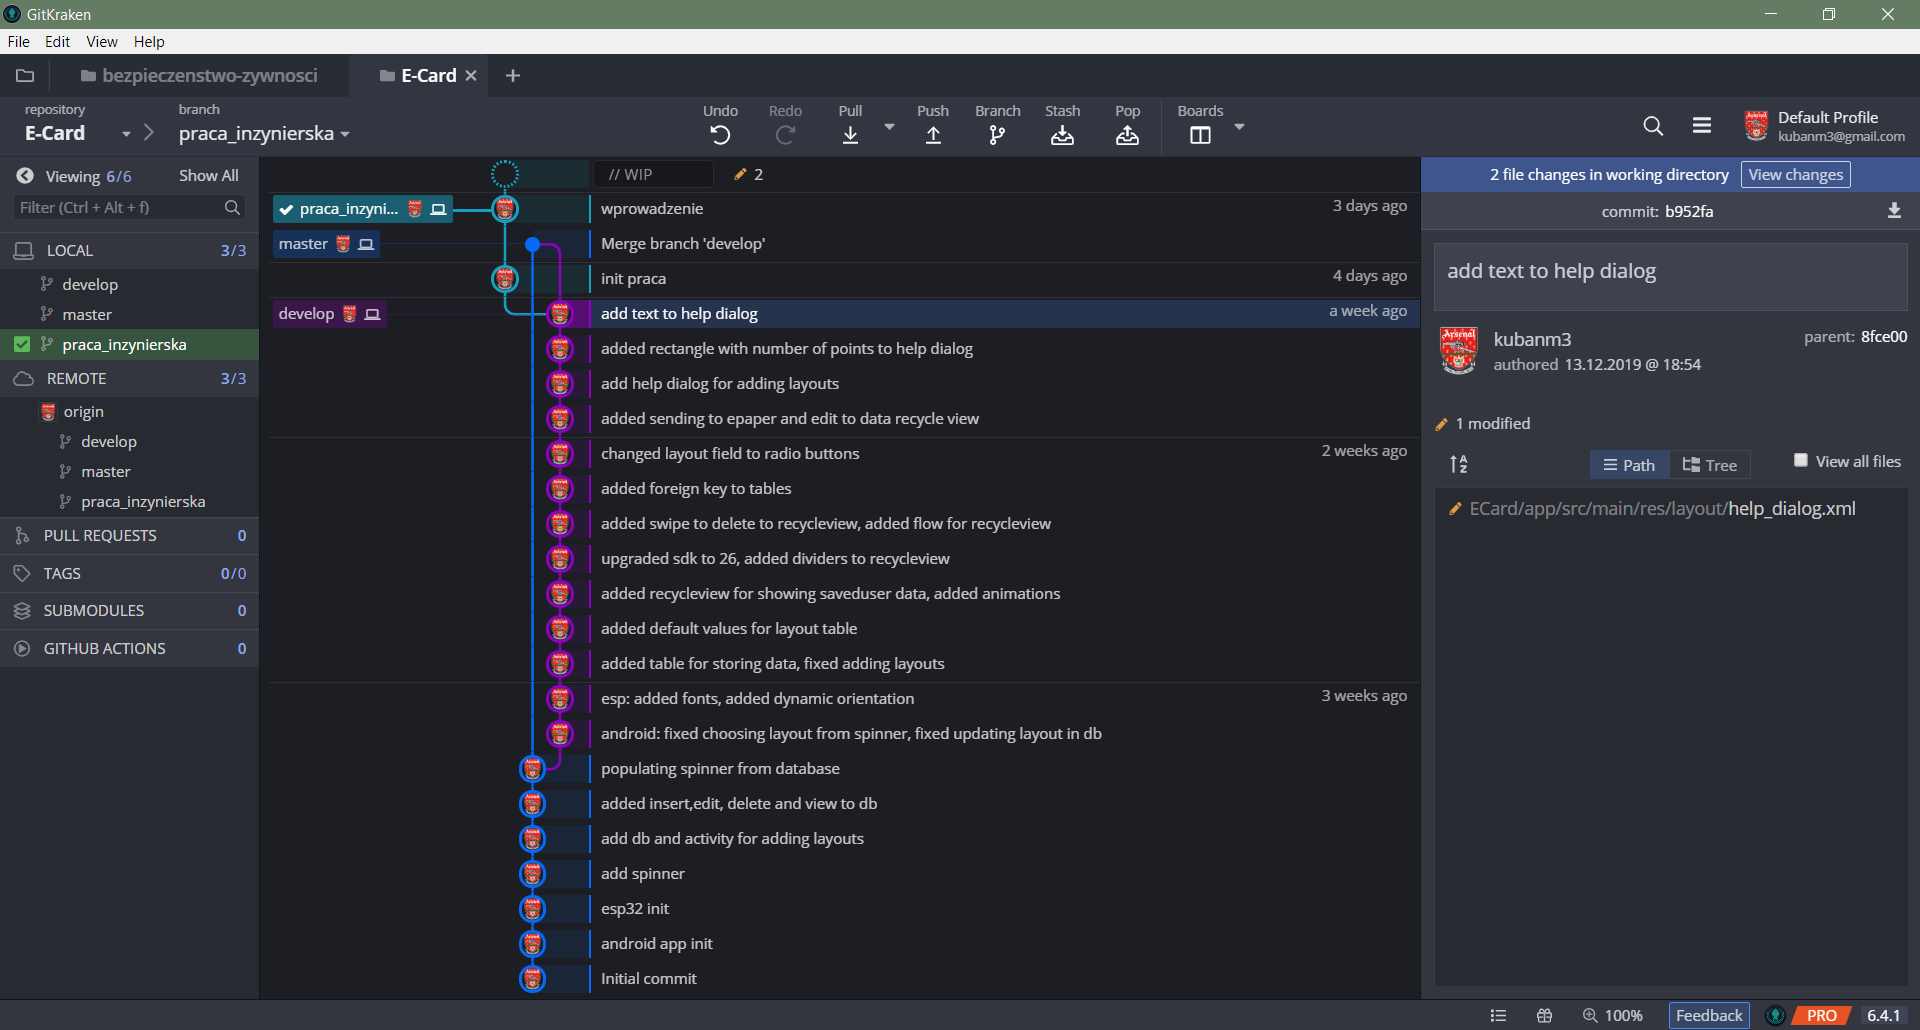
\includegraphics[width=1\textwidth]{images/rys2_gitkraken.png}
    		\caption{Repozytorium przedstawione w GitKraken}
            \label{fig:gitkraken}
    	\end{figure}
    		
    	W projektach, gdzie pracuje jednocześnie wiele osób, graficzna wizualizacja ułatwia kontrole nad wieloma gałęziami i zapanowanie nad projektem. Wykorzystana w projekcie wersja Pro GitKrakena dostępna jest w ramach GitHub Student Developer Pack\cite{githubpack}.
    	
    	\subsubsection{Arduino IDE}
    	Arduino IDE jest wieloplatformowym zintegrowanym środowiskiem deweloperskim napisanym w języku C oraz C++. Oparty jest na wolnej licencji GNU GPL v2.0. Wykorzystywane jest do pisania oraz wgrywania programów do kompatybilnych płytek Arduino. Możliwe jest również wykorzystanie go w celu wgrywania przygotowanego oprogramowania na płytki firm trzecich za pomocą dołączonych sterowników. 
    	
    	Programy pisane są w językach C oraz C++ używając specjalnych struktur kodowania. Udostępnionych do wykorzystania  jest wiele bibliotek obsługujących szeroką gamę czujników, serw czy wyświetlaczy.
    	
    	\begin{figure}[H]
    			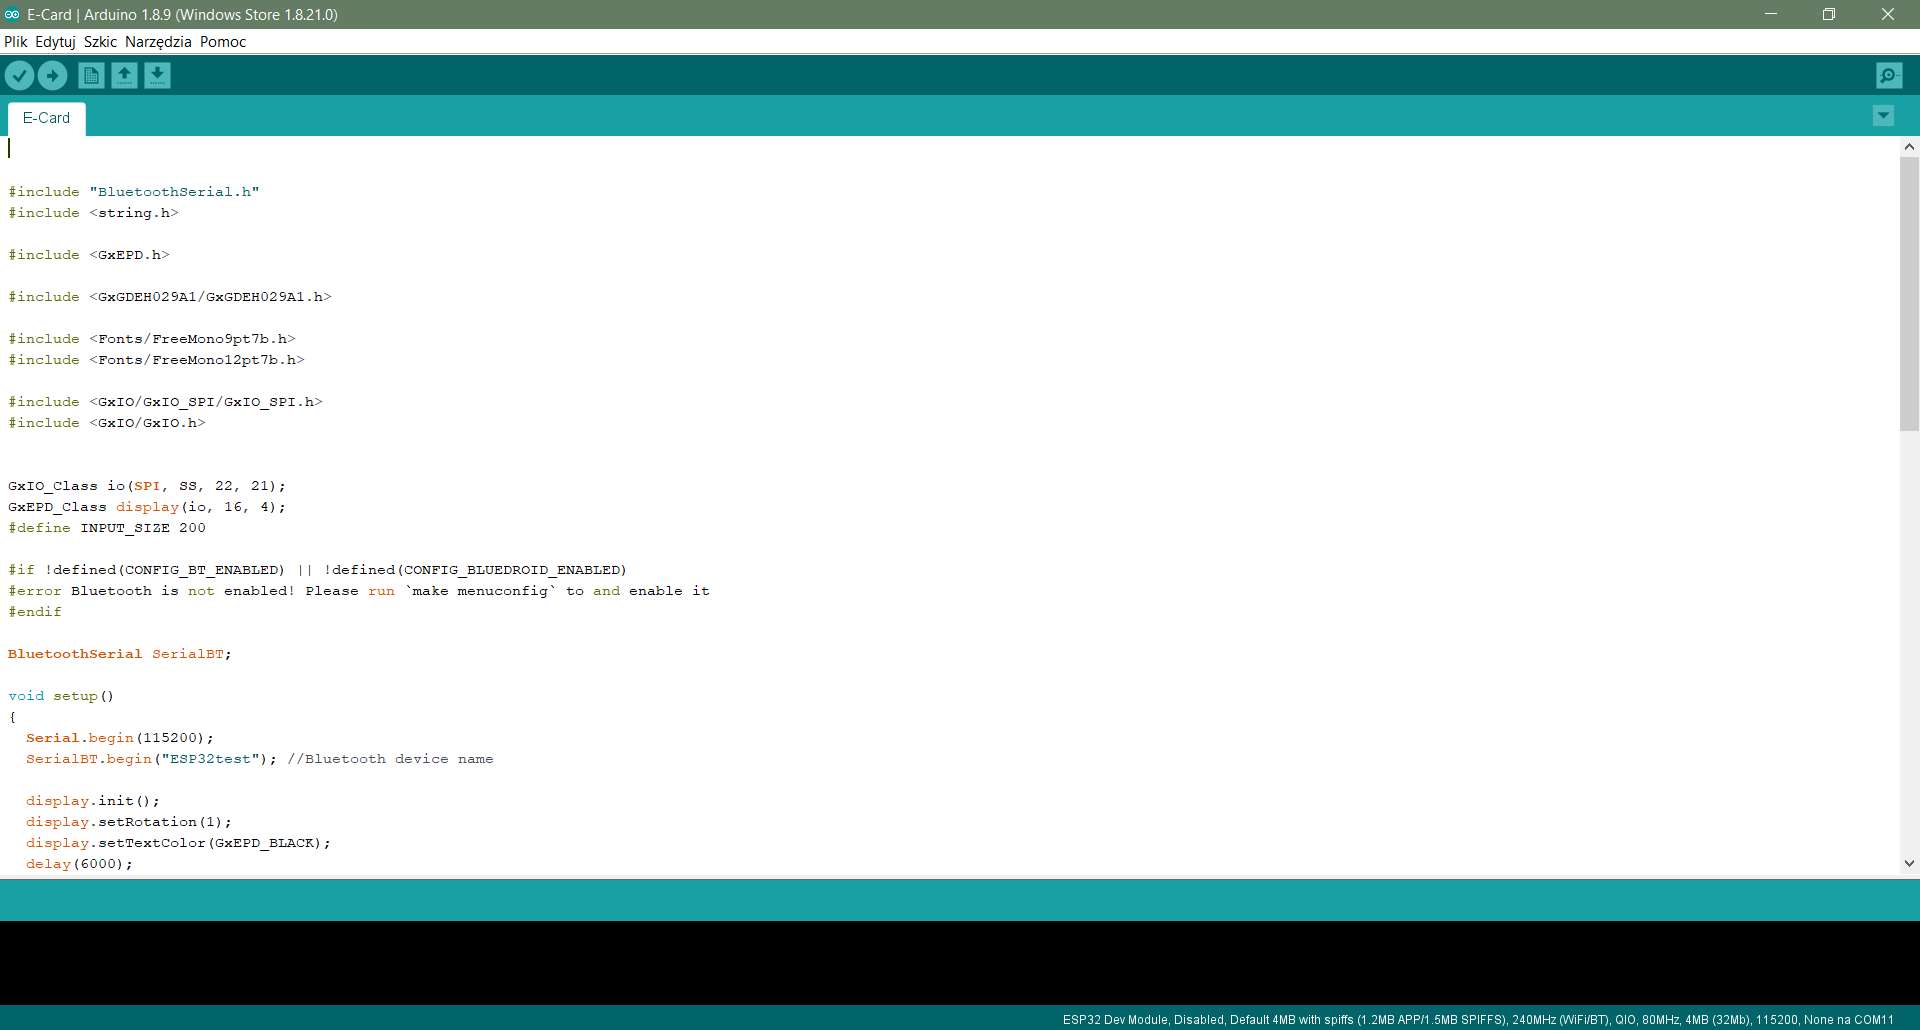
\includegraphics[width=1\textwidth]{images/rys3_arduino.png}
    			\caption{Widok Arduino IDE}
                \label{fig:arduinoide}
    	\end{figure}
    
    	Napisany przez użytkownika kod do działania potrzebuje tylko dwie podstawowe funkcje. Są nimi \textit{setup()} do rozpoczęcia działania i ustawienia początkowych parametrów oraz \textit{loop()}, która jest pętlą główną programu.
    	
    % 	\newpage
    	Środowisko zawiera trzy najważniejsze podprogramy, którymi są:
    	\begin{itemize}
    	\item Edytor kodu źródłowego — piszemy w nim nasz program. Zawiera takie funkcje jak sprawdzanie składni czy auto-formatowanie kodu.
    	\item Kompilator — wykonuje konwersje kodu wykonywalnego w plik tekstowy z szesnastkowym kodowaniem zrozumiałym przez mikrokontroler.
    	\item Loader — przesyła odpowiedni plik do Arduino.
    	\end{itemize}
    	
    	\subsection{Wykorzystane technologie}
    	\subsubsection{Java}
    	Java jest opartym na klasach, obiektowym językiem programowania. W programowaniu dla Androida wykorzystuje się przygotowane dla niego SDK\textit{ (z ang. Software development kit)}\cite{sdk}.
    	
    	W systemie Android cykl życia aplikacji wygląda inaczej niż w aplikacjach kontrolowanych przez JVM \textit{(ang. Java Virtual Machine)}\cite{jvm}. Nie występuje tutaj klasyczna metoda, jaką jest \textit{main(String[] args)}, mamy za to nowe metody w klasie aktywności, jakimi są onCreate, onPause, onDestroy, onRestart i inne. Metody te wykorzystywane są w różnych momentach działania aktywności, co możemy zobaczyć na rysunku numer \ref{fig:lifecycle}.
    
    	\begin{figure}[H]
    	        \centering
    			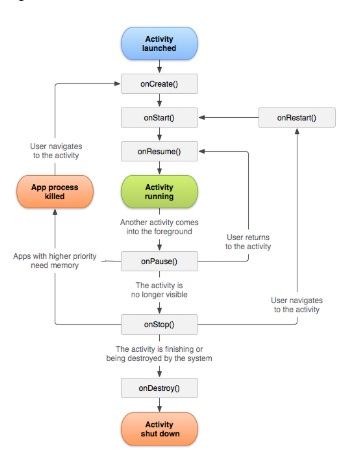
\includegraphics[width=7cm]{images/rys6_androidlifecycle.png}
    			\caption{Uproszczony ilustracja cyklu życia aktywności\cite{lifecycle}}
                \label{fig:lifecycle}
    	\end{figure}
    	
    	Metoda onCreate jest metodą uruchamianą jako pierwsza. W niej ustawiamy widok aktywności. Tutaj także przypisujemy kod do elementu, który chcemy, aby wykonywały się po interakcji z określoną kontrolką.
    	
    	Widoki aplikacji budowane są w wielu różnych plikach XML oraz klasach activity, gdzie istnieje możliwość tworzenia elementów programowo.
    	
    	W przeciwieństwie do \textit{JVM}, gdzie posiadamy pełną kontrolę nad cyklem życia procesu. W Androidzie aktywności są ciągle aktywne w tle, nawet po zamknięciu aplikacji przez użytkownika. To system steruje, kiedy aktywności zostają całkowicie wyłączone i usunięte z pamięci urządzenia. 
    	
    	Po zamknięciu aplikacje mogą ciągle działać w tle, jedynie zmniejszając część używanej przez siebie pamięci oraz zamykając niektóre z używanych procesów, jak na przykład połączenie Bluetooth, GPS czy łączność z internetem. Takie rozwiązanie ma sprzyjać szybkości i zmniejszeniu zużycia zasobów, podczas ponownego uruchamiania aplikacji. Dzięki czemu polepszać wykorzystanie baterii\cite{batterysave}.
    	
    	Więcej informacji na temat programowania w systemie Android można zaczerpnąć z książki \textit{Android Programming: The Big Nerd Ranch Guide (3rd Edition)}\cite{androidprogramming}.
    	
    	\subsubsection{SQLite}
    	SQLite jest relacyjną bazą danych dostępną na licencji \textit{public domain}\cite{publicdomain} zbudowaną w 2000 roku przez Richarda Hippa. SQLite implementuje mały rozmiarem (mniej niż 600KiB), szybki i samodzielny  silnik SQL \textit{(ang. Structured Query Language)}. Jest najczęściej używanym silnikiem baz danych na świecie. Występuje we wszystkich telefonach mobilnych oraz większości komputerów. Do działania nie potrzebuje dodatkowego procesu serwera, zapisuje i odczytuje dane bezpośrednio ze zwykłych dysków danych. Format plików jest uniwersalny, możliwe jest używanie i kopiowanie baz danych pomiędzy systemami 32 lub 64-bitowymi, lub wykorzystującymi architektury kolejności bajtów \textit{big-endian}, lub \textit{little-endian}\cite{endian}. SQLite jest starannie testowana przed wypuszczeniem każdej nowej wersji oprogramowania. Automatyczne testy osiągają 100 procent pokrycia rozgałęzień\cite{branchcoverage}. Na co dzień, SQLite jest wspierany przez międzynarodowy zespół programistów pracujących nad nim w pełnym wymiarze czasu. Kod źródłowy jest otwarty i dostępny dla każdego\cite{sqlite}.
    	
    	Szczegółowe informacje dotyczące SQLite i zasad jej działania oraz wykorzystanych technologii do produkcji tak wydajnej bazy danych można znaleźć w książce \textit{SQLite Forensics (2018)}\cite{sqliteforensics}. Zostały tam opisane z dokładnością co do bajta relacje pomiędzy danymi w wykonywanych zapytaniach.
    	
    	\subsubsection{Kod Arduino}
    	Kod Arduino pisany jest w C++ z dołączonymi do niego specjalnymi metodami i funkcjami. Został napisany specjalnie dla płytek Arduino i ich klonów. Ze względu na otwartą naturę projektu Arduino, biblioteki i inne źródła posiadają obszerną liczbę pozycji. Arduino posiada wiele wbudowanych bibliotek dostarczających podstawowe funkcjonalności większości elementów, które można podłączyć do płytki. 
    	
    	\begin{flushleft}
    	Programowanie na Arduino podzielone jest na dwie główne części:
    	\begin{enumerate}
    	    \item  
    	    \textbf{setup()}, ustalany jest tutaj początkowy stan Arduino po uruchomieniu. Wykonywany jest tylko jeden raz.	
    	    \begin{itemize}
    	        \item ustalany jest początkowy stan pinów
    	        \item przypisywane są zmienne
    	        \item tworzone są klasy
        	\end{itemize}
        	\item  
    	    \textbf{loop()}, zaczyna działać po skończeniu działania setup(). Uruchamiana jest w nieskończonej pętli, opisana jest w niej główna logika programu.
    	\end{enumerate}
    	
    	Każdy program napisany w Arduino opisać można w czterech głównych krokach:\cite{stepsarduino} 
    	\begin{enumerate}
    	    \item \textbf{Konfiguracja} — najczęściej opisana zostanie w \textit{setup()}. Wykonywana jest tylko raz w celu opisu pinów, przypisania zmiennych, kalibracji czujników.
    	    \item \textbf{Dane wejściowe} — po rozpoczęciu funkcji \textit{loop()} powinno nastąpić przypisanie przychodzących danych do zmiennych w celu dalszego wykorzystania. Zmienne mogą zostać użyte np. do wywołania instrukcji warunkowych lub przesłania dalej.
    	    \item \textbf{Obsługa danych} — konwersja danych do postaci, która będzie łatwiejsza do obsługi przez programistę np. przepisanie danych z portu szeregowego do tablic, po zastosowaniu odpowiednich algorytmów, czy przystosowanie ich do dalszego przesłania.
    	    \item \textbf{Dane wyjściowe} — np. wysłanie przygotowanych danych na port szeregowy do dalszej obróbki przez inne systemy lub przełączenie pinów na stany odpowiadające logice kodu.
    	\end{enumerate}
    	\end{flushleft}
    	
        Biblioteki wykorzystywane w programie Arduino składają się z plików źródłowych z rozszerzeniem \textit{.cpp}, oraz plików nagłówkowych \textit{.h}. Pliki nagłówkowe opisują strukturę biblioteki. Są w niej deklarowane wszystkie zmienne i funkcje wykorzystywane przez bibliotekę. W plikach źródłowych \textit{.cpp} zawarte są zaimplementowane kody funkcji.
        
    	\section{Opis i specyfikacja urządzenia}
    	Elektroniczna plakietka konfigurowana z urządzenia mobilnego składa się z dwóch części. Urządzenia mobilnego z zainstalowanym oprogramowaniem napisanym do obsługi tego projektu oraz urządzenia będącego fizyczną częścią projektu, składającego się z mikrokontrolera oraz wyświetlacza w technologii elektronicznego papieru.
    
        Przedstawię w tym rozdziale ogólny schemat projektu, wybrane podzespoły do jego wykonania. Opisane zostaną idea działania, jak również algorytm, według którego działa program mikrokontrolera.
        
        \subsection{Opis części fizycznej projektu}
        Urządzenie imitujące papierowy identyfikator zostało zaprojektowane do działania na mikrokontrolerze ESP32 firmy Espressif. Mikrokontroler posiada wbudowany moduł \textit{Bluetooth} BR/EDR \textit{(ang. Basic Rate/Enhanced Data Rate)}\cite{edr} oraz BLE \textit{(ang. Bluetooth Low Energy)}\cite{ble} do łączenia z urządzeniem mobilnym. Do wyświetlania przesyłanych danych używany jest wyświetlacz elektronicznego papieru firmy Waveshare, model WSR-09099, posiadający ekran o przekątnej 2.9 cala i rozdzielczości 296 × 128 pikseli. Możliwe jest jednak wykorzystanie dowolnego wyświetlacza 
        pracującego w szeregowym interfejsie SPI 4-line i obsługiwanego przez biblioteki \textit{GxEPD}\cite{gxepd}.
        
        \subsubsection{Schemat blokowy projektu}
        Na rysunku numer \ref{fig:block}. przedstawiony został schemat blokowy wykonanego projektu. Projekt posiada cztery główne bloki, jakimi są urządzenie mobilne, mikrokontroler ESP32 z wbudowanym modułem Bluetooth oraz wyświetlacz e-papieru.
        \begin{figure}[H]
    	        \centering
    			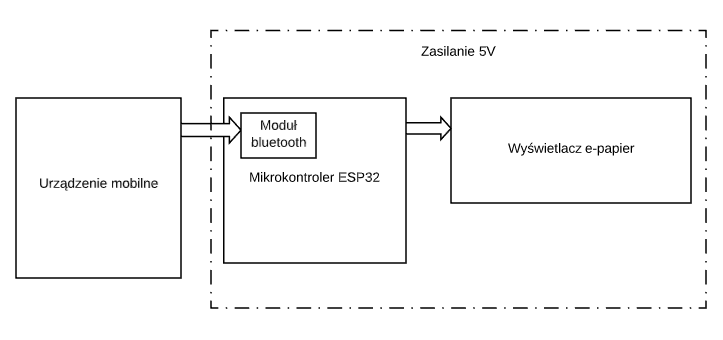
\includegraphics[width=13cm]{images/rys_7schemat_blokowy.png}
    			\caption{Schemat blokowy projektu}
                \label{fig:block}
    	\end{figure}
    	
        \subsubsection{Opis poszczególnych bloków układu}
        \textbf{Urządzenie mobilne} wykorzystane w obsłudze wyświetlacza papieru elektronicznego musi posiadać wersje systemu Android OS w wersji co najmniej 4.0.3 (\textit{Ice Cream Sandwich})\cite{ics}, posiadającą API w wersji 15\cite{api}. 
        
        Kolejnym wymogiem korzystania z pełnej funkcjonalności projektu, jest obecność modułu Bluetooth w urządzeniu mobilnym. Bez jego obecności niemożliwe staje się przesłanie danych do mikrokontrolera, a zarazem wyświetlenie ich na papierze elektronicznym.
        
    	\textbf{Mikrokontrolerem}, użytym w projekcie jest 32-bitowy ESP32 firmy Espressif. Pracuje on przy 3.3V napięcia roboczego. Do zbudowania prototypu posłużono się kitem developerskim ESP32-DevKitC. Posiada on wbudowany port Micro-USB do zasilania urządzenia oraz możliwość współpracy ze środowiskiem programistycznym Arduino. Z tego samego portu USB zasilany jest również wyświetlacz papieru elektronicznego. Kit posiada 4MB pamięci flash\cite{flash}. Mamy do dyspozycji również trzydzieści osiem wyprowadzeń, z czego dwadzieścia trzy są wyprowadzeniami GPIO \textit{(ang. general-purpose input/output)}. Piny te wykorzystywane są w komunikacji pomiędzy mikroprocesorem a urządzeniami peryferyjnymi.
    	\begin{figure}[H]
    	        \centering
    			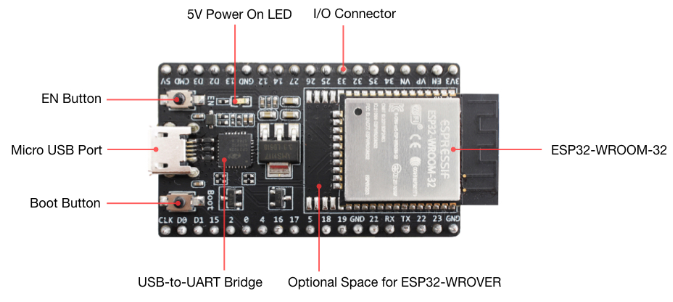
\includegraphics[width=9cm]{images/rys8_devkit.png}
    			\caption{Schemat ESP32-DevKitC\cite{devkit}}
                \label{fig:devkit}
    	\end{figure}
    	
    	Zadaniem mikrokontrolera jest odbieranie danych z połączonego urządzenia mobilnego, następnie przetworzenie ich i przesłanie do wyświetlenia na podłączonym wyświetlaczu e-papier.
    
        \textbf{Wyświetlacz papieru elektronicznego} jest to 2.9-calowy ekran firmy Waveshare. Przystosowany jest do pracy w dwóch napięciach roboczych 3.3V oraz 5V. Zasilany jest przez wyjście 3.3V dostępne w ESP32. Jest w stanie wyświetlać dane w dwóch kolorach (białym i czarnym) z czasem potrzebnym do pełnego odświeżenia wyświetlacza równym w przybliżeniu 2 sekundy\cite{waveshare}.
        
        Wykorzystane piny do połączenia wyświetlacza z mikrokontrolerem: 
        \begin{itemize}
            \item \textbf{VCC, GND} — zostały połączone z wyjściami 3.3V oraz GND mikrokontrolera. Piny te dostarczają zasilanie wyświetlaczowi.
            \item \textbf{DIN, CLK, CS} — są to piny wykorzystywane przez interfejs szeregowy SPI. CLK jest linią zegara. Przez DIN dane przesyłane są z mikrokontrolera (mastera) do wyświetlacza (slave). CS używany jest do wyboru aktywnego urządzenia (stan niski), w naszym projekcie podłączone mamy tylko jedno urządzenie więc jest ono zawsze aktywne.
            \item \textbf{DC} — wybór przesyłania danych lub komend do wyświetlacza. Stan wysoki dla danych, stan niski dla komend.
            \item \textbf{RST} — zewnętrzny reset, aktywowany stanem niskim.
            \item \textbf{BUSY}  — linia wyjściowa wyświetlacza wykorzystywana do przesyłania informacji do mikrokontrolera o stanie zajętości wyświetlacza. Przy stanie aktywnym (aktywność przy niskim stanie) wyświetlacz nie będzie reagował na komendy przesłane przez mikrokontroler. 
        \end{itemize}
        
        \subsection{Opis części programowej mikrokontrolera}
    	Program sterujący działaniem mikrokontrolera został napisany w języku C++ w zintegrowanym środowisku programistycznym Arduino IDE, które dostępne jest za darmo na licencji GNU General Public License. Program jest kompilowany, a następnie przesyłany do mikrokontrolera za pomocą wbudowanego w kit deweloperski programatora AVRISP mk2.
   
    	\subsubsection{Zasada działania}

        Program opiera się na dwóch częściach. Pierwsza część odpowiedzialna jest za upewnienie się, że moduł Bluetooth dostępny w urządzeniu sterującym działa prawidłowo. Obsługa modułu oparta jest na kodzie napisanym przez Espressif i udostępnianym na licencji Apache License, Version 2.0.

    \begin{lstlisting}[language=C++, caption=Sprawdzenie poprawności działania Bluetooth]
#if !defined(CONFIG_BT_ENABLED) || !defined(CONFIG_BLUEDROID_ENABLED)
#error Bluetooth is not enabled! Please run `make menuconfig` to and enable it
#endif\end{lstlisting}
    
    	Następnym krokiem jest zrobienie instancji klasy odpowiadającej za działanie modułu Bluetooth i inicjalizacja komunikacji szeregowej urządzenia sterującego z prędkością transmisji ustawioną na 115200 baudów\cite{baud}. Później inicjowane jest szeregowe połączenie urządzenia Bluetooth i rozpoczęte jest rozgłaszanie podanej nazwy programowanego urządzenia. Po wykonaniu powyższych zadań program przechodzi do kolejnej części.
    	
    	Druga część programu jest wykonywana w nieskończonej pętli. Schemat działania pętli przedstawiony jest na rysunku numer \ref{fig:petlamikrokontrolera}. W niej tworzone są potrzebne do działania programu zmienne i przypisywane są im wartości startowe, które w dalszej części kodu będą używane i modyfikowane. 
    	
    	Głównym zadaniem pętli jest nasłuchiwanie portu szeregowego modułu Bluetooth. Otrzymane na porcie RX dane, zapisywane są do zmiennych. W kolejnym kroku wykonywanym przez nasz program, dane te przetwarzane są do postaci, którą można wysłać i wyświetlić na wyświetlaczu papieru elektronicznego. Wykorzystywana jest do tego funkcja dostępna w języku C jaką jest \textit{strtok}\cite{strtok}. Funkcja ta rozdziela otrzymane dane z portu szeregowego Bluetooth na słowa. \label{petladekod}Ogranicznikiem, a zarazem argumentem, który musi być podany w funkcji, jest \textit{";"}. Po jego wykryciu następuje podział danych przesłanych z urządzenia mobilnego.
    	
    	Przy pierwszym wykonaniu, funkcja oczekuje łańcucha znaków odebranych z urządzenia mobilnego jako pierwszy argument, oraz znaku służącego do podziału (ogranicznika) jako drugi argument. Kolejne wywołania \textit{strtok} wykonywane są w pętli działającej do otrzymania wskaźnika zerowego, który jest zwracany przez funkcję po wystąpieniu końca łańcucha znaków. Funkcja zwraca wskaźnik do następnego słowa, jeżeli występowało słowo poprzednie. W wypadku gdy wystąpi koniec łańcucha znaków, zwracany jest wskaźnik zerowy. W pętli wydzielone słowo jest kopiowane, a następnie zostaje wpisane do utworzonej wcześniej tablicy. Za kopiowanie i przepisanie słowa do tablicy odpowiada funkcja \textit{strcpy}\cite{strcpy}, która jest dostępna w języku C, w klasie string.h. Następnie po raz kolejny wywoływana jest funkcja \textit{strtok}, tym razem pierwszym argumentem musi być wskaźnik zerowy. Funkcja sama ustawia się na końcu poprzedniego słowa jako początkowe miejsce do ponownego skanowania w celu wykrycia znaku specjalnego. Pętla kończy się po wykryciu przez \textit{strtok} znaku \textit{null}, czyli znaku sterującego o wartości liczbowej 0, informującego o braku informacji\cite{null} i zwróceniu przez nią wskaźnika zerowego. Pseudokod pętli przedstawiony jest w algorytmie numer \ref{lst:petlaprzepisujaca}.
    \begin{lstlisting}[language=C++, label={lst:petlaprzepisujaca}, caption=Działanie pętli przepisującej otrzymane dane do tablicy]
char *ptr = strtok(input, ";");
while (ptr != NULL) {
  strcpy(ch_arr[i], ptr);
  ptr = strtok(NULL, ";");
  i++;
}\end{lstlisting}
    
    	Posiadając wszystkie dane, potrzebne do prawidłowego wyświetlenia na ekranie wyświetlacza, program rozpoczyna przesyłanie ich na ekran. Pierwszym krokiem jest ustawienie orientacji ekranu. Następnie ustawiana jest wielkość czcionki oraz współrzędne pozycji startowej kursora, skąd rozpoczyna się rysowanie tekstu na wyświetlaczu papieru elektronicznego. Wielkość czcionki oraz współrzędne są ustalane dla każdej przesłanej informacji z osobna.
    	
    	\subsubsection{Schemat blokowy pętli programu mikrokontrolera}
    	Na rysunku numer \ref{fig:petlamikrokontrolera}. przedstawiony został schemat blokowy działania głównej pętli programu mikrokontrolera ESP32. Przedstawiono tam kroki wykonywane przed wejściem do pętli oraz działanie pętli.
 
    	\begin{figure}[H]
    	        \centering
    			\includegraphics[width=10.5cm]{images/rys10_petlamikro.png}
    			\caption{Schemat blokowy pętli programu mikrokontrolera}
                \label{fig:petlamikrokontrolera}
    	\end{figure}
    	
    	\section{Opis aplikacji}
    	Aplikacja na urządzenie mobilne została napisana dla systemu mobilnego Android w środowisku Android Studio firmy Google. Środowisko to jest dostosowane do budowy aplikacji na system Android. Aplikację napisano w języku Java. Minimalna wersja API to 15. Jest ona obecna w systemie Android od wersji 4.0.3 \textit{Ice Cream Sandwich} z czerwca 2012 roku.
    	
    	Program zaprojektowano zgodnie ze wzorcem programowania obiektowego \textit{(Object Oriented Programming)}\cite{oop}, w którym kod podzielony jest na części, które są łatwiejsze w utrzymaniu i konserwacji. Każda część jest samodzielna w swojej funkcjonalności, zarazem możliwe jest wykorzystanie jej przez inne programy działające w aplikacji. Wszystkie części działają wspólnie, tworząc całość aplikacji. Części te nazywane są obiektami. 
    	
    	Aplikacja posiada cztery aktywności odpowiadające za różne funkcjonalności. Do przechowywania danych użyto relacyjnej bazy danych SQLite. W aplikacji można przechowywać zapisane dane do wyświetlenia na wyświetlaczu, jak również przygotowane i zapisane układy wyświetlania.
    	
    	\subsection{Podział na klasy}
    	Aplikacja składa się z kilku klas, są one odpowiedzialne za np. wyświetlanie widoków oraz obsługę ich funkcjonalności czy obsługę bazy danych. Występuje klasa adaptera danych widoku listy oraz istnieje klasa bazowa, z której dziedziczy reszty obecnych w aplikacji klas.
    	
    	Klasy występujące w aplikacji i ich skrócony opis:
    	\begin{itemize}
    	    \item \textit{DeviceList} — klasa odpowiada za sprawdzanie, czy urządzenie jest wyposażone w moduł Bluetooth i czy jest on włączony. Po spełnieniu tych warunków wyświetla sparowane z urządzeniem mobilnym urządzenia Bluetooth. Po wybraniu odpowiedniego urządzenia przesyła jego adres Bluetooth \textit{(ang. Bluetooth Device Address)}\cite{bdaddr} do kolejnej klasy.
    	    \item \textit{DataControl} — po stworzeniu klasy następuje próba połączenia z urządzeniem, którego adres Bluetooth został otrzymany. Urządzenie, z którym próbowane jest nawiązanie połączenia, nie może być w tym samym czasie połączone. W tej samej klasie pokazany jest widok, z którego można uzupełnić dane do wyświetlenia na papierze elektronicznym. Możliwe jest również wysłanie danych na urządzenie poprzez ustanowioną łączność Bluetooth lub zapisanie ich do bazy danych w celu późniejszego wykorzystania. Została w tym miejscu również zaimplementowana funkcjonalność rozłączenia z urządzeniem Bluetooth.
    	    \item \textit{DatabaseHelper} — jest to klasa pomocnicza do obsługi bazy danych SQLite. Przygotowywane i wykonywane są w niej skrypty do tworzenia tabeli danych oraz tabeli układów. Tabela, w której przechowywane są układy jest tutaj również uzupełniana wartościami domyślnymi. Zamieszczone są w niej metody do obsługi tabel, takie jak pobieranie, edycja i usuwanie rekordów.
    	    \item \textit{DataList} — klasa w której wyświetlane są rekordy z tabeli zawierającej zapisane dane. Dane te można przesyłać na wyświetlacz papieru elektronicznego. Po przesunięciu wybranego rekordu mamy możliwość usunięcia go lub przesłania do widoku, gdzie można nim sterować.
    	    \item\textit{DataAdapter} — jest to klasa pomocnicza dla klasy DataList. Odpowiada ona za poprawne wyświetlanie danych pobranych z bazy danych na adapterze widoku liście.
    	    \item \textit{AddLayout} — klasa odpowiada za dodawanie nowych układów do wyświetlania danych na ekranie papieru elektronicznego. Posiada również metody edycji i usuwania układów danych. Jest tutaj również zaimplementowany prosty dialog pomagający w projektowaniu nowych układów danych.
    	    \item \textit{DynamicSquareLayout} — klasa odpowiada za obliczanie i ustawianie proporcji pomocniczego widoku wyświetlacza, który znajduje się w dialogu pomocy, zaimplementowanym w klasie \textit{AddLayout}. Proporcje te odpowiadają fizycznym rozmiarom podłączonego wyświetlacza. Wysokość i szerokość wyświetlacza prezentowanego w dialogu dobierane są w taki sposób, aby jego szerokość była równa 80-ciu procentom szerokości ekranu urządzenia mobilnego.
    	    \item \textit{BaseActivity} — jest klasą bazową aplikacji. Z niej dziedziczą inne klasy. Napisane zostały w niej metody wykorzystywane we wszystkich widokach, jak również metody, które przesyłają dane pomiędzy kilkoma klasami. Metodą wykorzystywaną przez wszystkie widoki i napisaną w tej klasie, jest metoda odpowiedzialna za wyświetlanie wszystkich dostępnych i zapisanych w tabeli układów danych.
    	\end{itemize}
    
        \subsubsection{Baza danych}
        W aplikacji istnieje możliwość przechowywania rekordów zapisanych wpisów z danymi personalnymi oraz układów danych. Obsługa zapisanych danych wykonywana jest w relacyjnej bazie danych SQLite. Baza posiada dwie tabele połączone ze sobą kluczem obcym. Na rysunku numer \ref{fig:database}. można zobaczyć diagram związków encji bazy danych. 
        
        Kolumna id występująca w tabeli \textit{layouts} jest kluczem głównym tej tabeli jest również wykorzystywana jako klucz obcy tabeli \textit{data}. 
        
        \begin{figure}[H]
    	        \centering
    			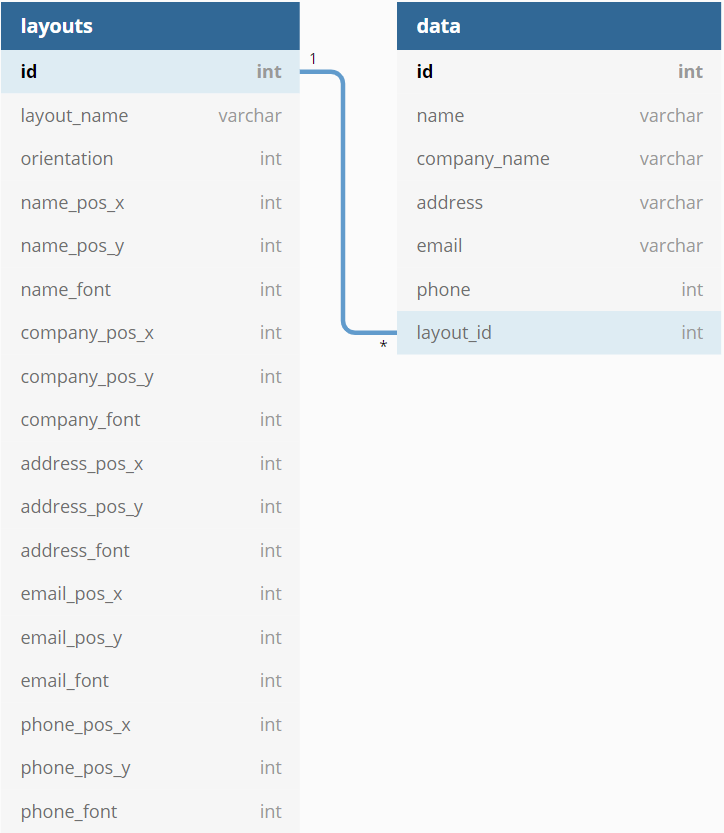
\includegraphics[width=12cm]{images/rys_11baza.png}
    			\caption{Diagram związków encji bazy danych}
                \label{fig:database}
    	\end{figure}
    	
        Relacja występująca pomiędzy tabelami to relacja jeden do wielu (1: N). Oznacza to, że jeden rekord tabeli \textit{layouts} może być wykorzystany przez wiele rekordów w tabeli \textit{data}. Z drugiej strony, pojedynczy wpis w tabeli \textit{data} może posiadać tylko jeden layout. Dzięki takiemu połączeniu SQLite zapewnia poprawność działania bazy danych, uniemożliwiając usunięcie wpisów wykorzystywanych przez inne tabele. 
        
        W zaprojektowanej dla projektu bazie danych niemożliwe będzie usunięcie rekordu tabeli \textit{layouts}, gdy jego klucz główny \textit{id} jest obecny w kolumnie \textit{layout\_id} tabeli \textit{data}, który jest kluczem obcym tej tabeli. Po wykryciu przez bazę danych takiego zachowania wyrzucany jest błąd, który następnie obsługiwany zostaje przez aplikację w celu przekazania użytkownikowi informacji o niepożądanej akcji.
    	
    	\subsubsection{Połączenie Bluetooth}
    	Połączenie, obsługa i komunikacja Bluetooth jest zarządzana poprzez pakiet dostępny dla systemu Android, jakim jest \textit{android.bluetooth}\cite{android.bluetooth}. W projekcie wykorzystywana jest funkcjonalność wyszukiwania dostępnych urządzeń, nawiązywania połączenia oraz przesyłania danych. Schemat blokowy przedstawiający nawiązywanie połączenia pomiędzy urządzeniem mobilnym a urządzeniem wyświetlającym, przedstawiony jest na rysunku numer \ref{fig:btconnect}. 
    	
    	Pierwszym krokiem nawiązania komunikacji poprzez adapter Bluetooth jest sprawdzenie, czy moduł ten, jest obecny w urządzeniu mobilnym. W przypadku gdy urządzenie mobilne nie posiada adaptera Bluetooth, aplikacja blokuje większość funkcji, pozostawiając jedynie możliwość przeglądania i dodawania nowych układów danych. 
    	
    	Przy pozytywnym stwierdzeniu obecności modułu, można przejść do dalszych kroków. Następnym etapem jest sprawdzenie, czy moduł Bluetooth jest włączony. W przypadku gdy Bluetooth jest wyłączony, następuje wyświetlenie prośby o jego włączenie. Później pobierana jest lista sparowanych z urządzeniem mobilnym urządzeń Bluetooth. Wykorzystywana jest do tego metoda \textit{getBondedDevices}\cite{bonded} dostępna w klasie \textit{BluetoothAdapter}. Metoda ta zwraca zbiór obiektów sparowanych z lokalnym dla aplikacji adapterem Bluetooth. Po wybraniu urządzenia pobierany jest jego adres BD\_ADDR i nawiązywana jest próba połączenia. Sprawdzana jest dostępność urządzenia, następnie utworzone zostaje połączenie \textit{RFCOMM}\cite{rfcomm}. Po wykonaniu poprzedzających czynności możliwe jest nawiązanie połączenia pomiędzy urządzeniami. Połączone urządzenia dysponują szeregowym połączeniem, po którym można przesyłać dane.
    	
    	\begin{figure}[H]
    	        \centering
    			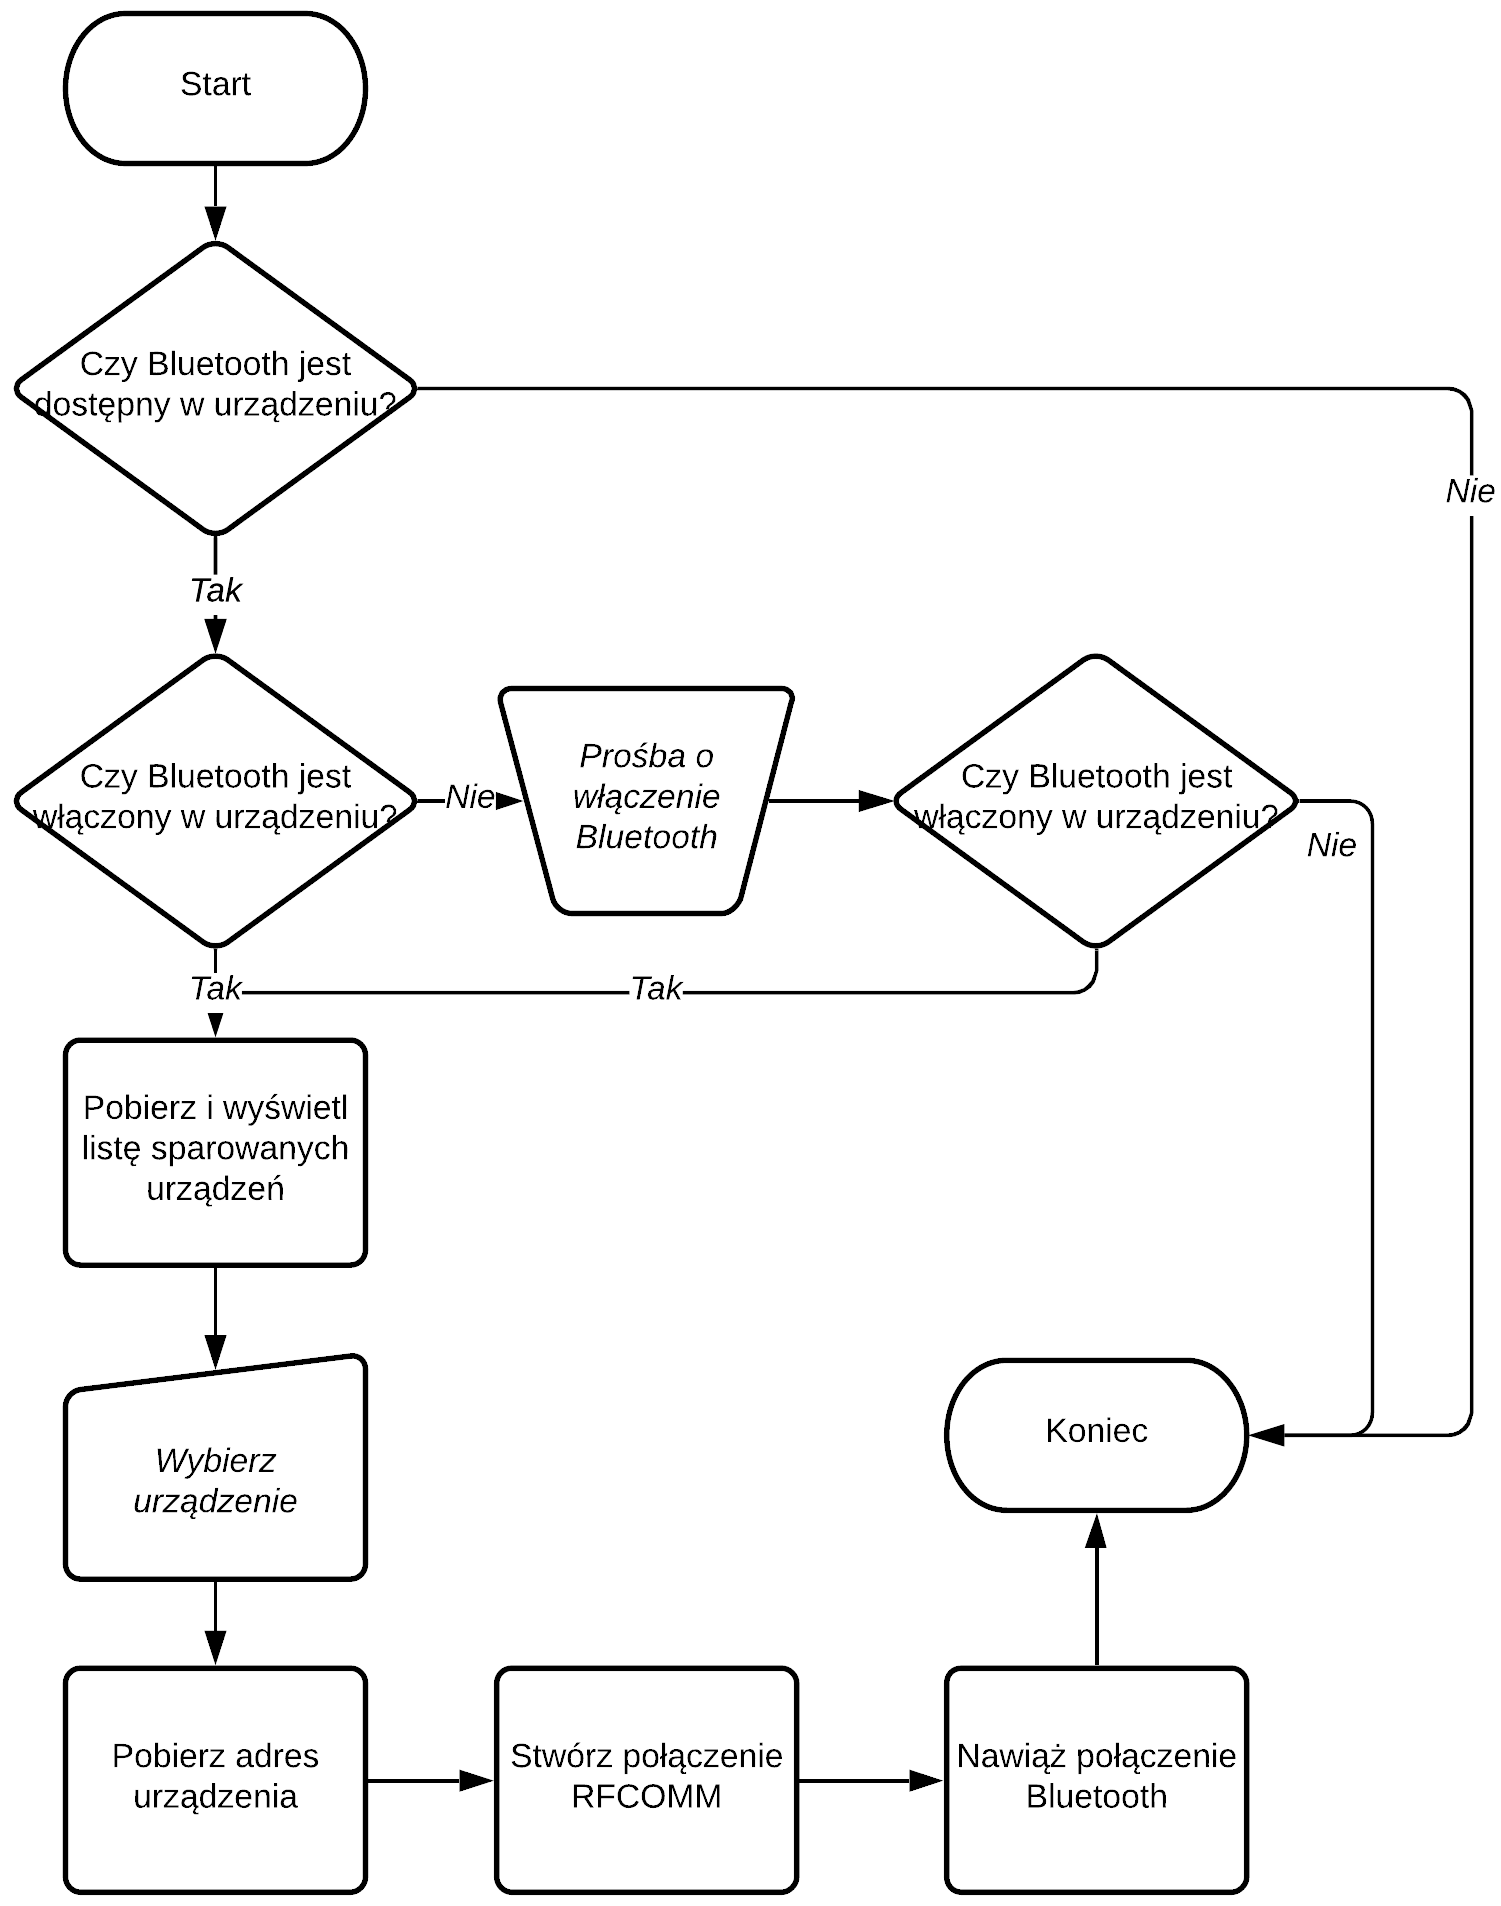
\includegraphics[width=12cm]{images/rys_12bluetoothconnection.png}
    			\caption{Schemat blokowy nawiązywania połączenia Bluetooth}
                \label{fig:btconnect}
    	\end{figure}
    	
    	\subsection{Transmisja danych}
    	Obsługa przesyłania danych realizowana jest poprzez klasę \textit{BluetoothSocket}. Używając metody \textit{getOutputStream}\cite{outputstream}, otwarty zostaje strumień wyjścia, za pomocą którego można przesyłać dane binarne. Przed przesłaniem, dane pobierane są z przygotowanych na widoku pól edycji, do których były wcześniej wpisane lub przesłane z bazy danych. Dane te przed wysłaniem są przystosowywane do poprawnego odbioru przez mikrokontroler. Po każdym słowie dodawany jest znak specjalny \textit{";"}, który w programie mikrokontrolera używany jest do rozróżniania ciągu znaków. Algorytm służący do dekodowania odebranych przez urządzenie mobilne danych, obecny jest w mikrokontrolerze i został opisany w części \ref{petladekod} \textit{Zasada działania}.
    	
    	Transmisja danych możliwa jest tylko w wypadku gdy gniazdo Bluetooth jest połączone z urządzeniem docelowym.
    	
    	\section{Instrukcja obsługi}
    	W tej części pracy, opisane zostaną wszystkie działania konieczne do poprawnego uruchomienia urządzenia identyfikatora oraz urządzenia mobilnego w celu wykorzystania wszystkich funkcjonalności przygotowanych dla aplikacji mobilnej.
    	
    	\subsection{Uruchomienie elektronicznej plakietki}
    	Plakietka do działania potrzebuje zasilania 3.3V, które należy dostarczyć za pomocą wejścia USB, znajdującego się w kicie deweloperskim mikrokontrolera. Prototyp zasilany był z zewnętrznej baterii, co zapewniało mu możliwość przenoszenia. Po dostarczeniu zasilania i przy wgranym na mikrokontroler oprogramowaniu plakietka jest bezobsługowa.
    	
    	\subsection{Obsługa aplikacji mobilnej}
    	Przed pierwszym uruchomieniem aplikacji należy sparować urządzenie mobilne i elektroniczną plakietkę ze sobą za pomocą łączności Bluetooth. Po upewnieniu się, że łączność Bluetooth w naszym urządzeniu mobilnym jest włączona, można przejść do ustawień, gdzie należy znaleźć stronę z ustawieniami połączeń Bluetooth. Po kliknięciu przycisku wyszukiwania urządzeń, wyświetlone zostaną dostępne do połączenia urządzenia. Należy znaleźć urządzenie o nazwie \textit{ESP32test} i połączyć się z nim. Połączenie nie wymaga podania hasła lub pinu. Po sparowaniu urządzeń można przejść do uruchomienia aplikacji. 
    	
    	Po instalacji i pierwszym uruchomieniu aplikacja tworzy bazę danych i uzupełnia ją domyślnymi układami. 
    	Przy pierwszym i każdym następnym włączeniu, sprawdzana jest obecność modułu Bluetooth. W przypadku braku modułu, funkcjonalności aplikacji zostają ograniczone. Następnie sprawdzane jest, czy moduł Bluetooth jest uruchomiony. Przy wyłączonym module aplikacja wyświetli dialog proszący o włączenie modułu Bluetooth. Ekran tego dialogu został przedstawiony na rysunku numer \ref{fig:bton}.
    	
    	\begin{figure}[H]
    	\centering
    	\begin{minipage}{.5\textwidth}
    	    \centering
    	    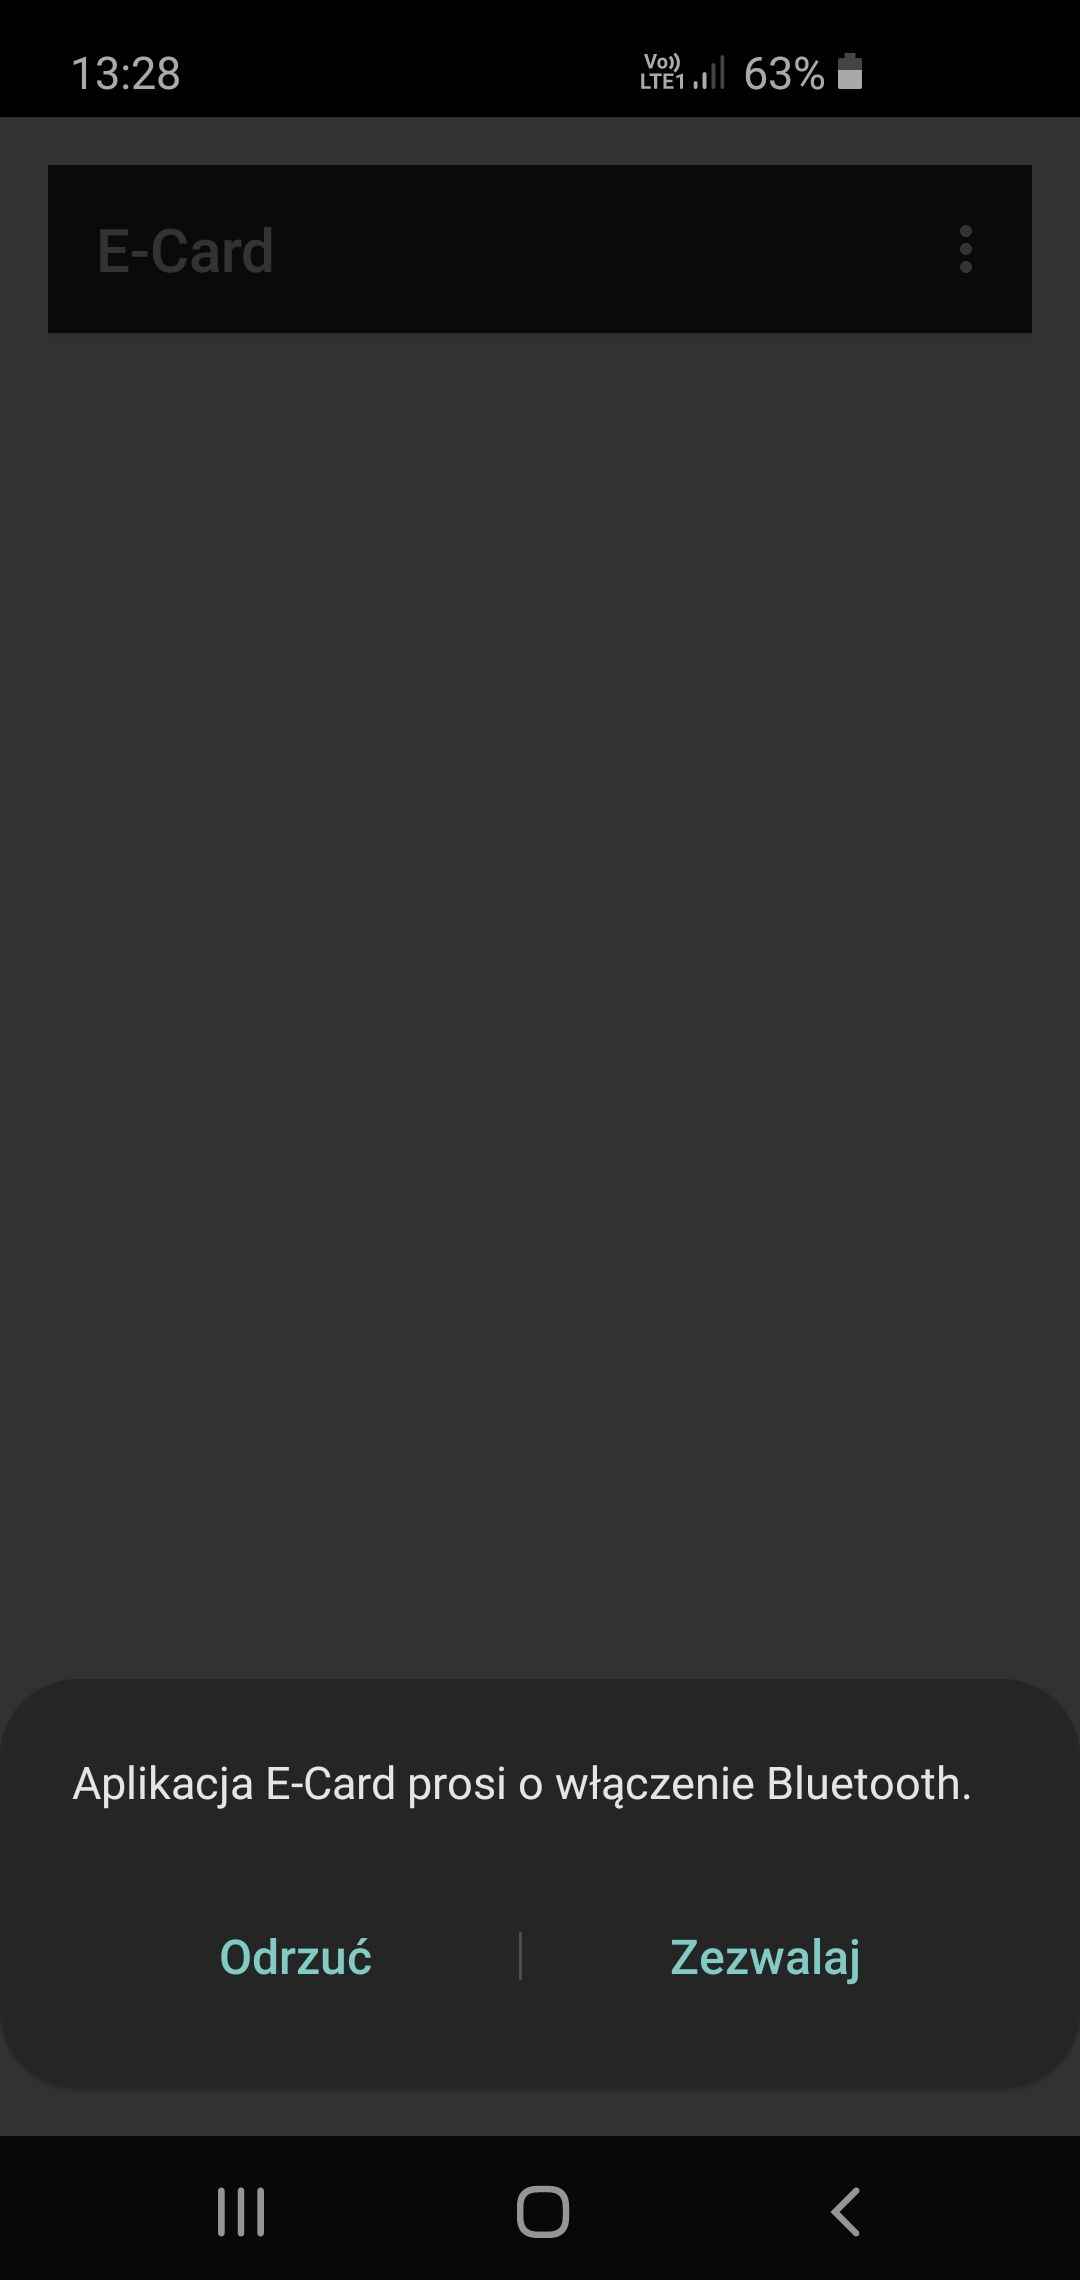
\includegraphics[width=6cm]{images/rys_13bluetoothdialog.jpg}
    	    \captionof{figure}{Dialog proszący \newline o włączenie Bluetooth}
            \label{fig:bton}
        \end{minipage}%
        \begin{minipage}{.5\textwidth}
            \centering
    	    \includegraphics[width=6cm]{images/rys_14devicelist.jpg}
    	    \captionof{figure}{Ekran wyświetlający listę sparowanych urządzeń}
            \label{fig:btdevices}
        \end{minipage}
    	\end{figure}
    	\vspace{.5cm}
    	
    	Na rysunku numer \ref{fig:btdevices}. przedstawiona jest sytuacja po włączeniu adaptera Bluetooth. Wyświetlona zostaje wtedy lista urządzeń, z którymi można się połączyć. Po wybraniu nazwy prototypu, którą jest \textit{ESP32test}, aplikacja przechodzi do widoku, w którym można sterować danymi.
    	\newpage
    	Sterowanie danymi odbywa się w widoku pokazanym na rysunku numer \ref{fig:datacontrol}. Widok ten oferuje funkcjonalności przesyłania danych do identyfikatora oraz zapisu w bazie danych. Informacje, jakie można przesłać na elektroniczną plakietkę to:
    	\begin{itemize}
    	    \item Imię i nazwisko
    	    \item Nazwa firmy
    	    \item Adres firmy
    	    \item Adres poczty elektronicznej
    	    \item Numer telefonu
    	\end{itemize}
    	
    	\begin{figure}[H]
    	        \centering
    			\includegraphics[width=6cm]{images/rys_15datacontrol.jpg}
    			\caption{Ekran umożliwiający sterowanie danymi}
                \label{fig:datacontrol}
    	\end{figure}
    	
    	Aplikacja posiada również widok, na którym prezentowane są zapisane w bazie danych informacje do wyświetlania na identyfikatorze. Z tego samego okna można usuwać i modyfikować zapisane rekordy. Widok z akcjami usuwania i modyfikacji jest pokazany na rysunku \ref{fig:datadelete}. i \ref{fig:dataedit}.
    	
    	\begin{figure}[H]
    	\centering
    	\begin{minipage}{.5\textwidth}
    	    \centering
    	    \includegraphics[width=6cm]{images/rys_16delete.jpg}
    	    \captionof{figure}{Lista danych — usuwanie}
            \label{fig:datadelete}
        \end{minipage}%
        \begin{minipage}{.5\textwidth}
            \centering
    	    \includegraphics[width=6cm]{images/rys_17edit.jpg}
    	    \captionof{figure}{Lista danych — edycja}
            \label{fig:dataedit}
        \end{minipage}
    	\end{figure}
    	
    	Po wykonaniu akcji edycji, przesunięciu wiersza w prawo, następuje przejście do ekranu sterowania danymi, gdzie informacje z bazy danych zostaną wpisane do pól edycyjnych. Następnie istnieje możliwość edycji lub wysłania ich na urządzenie wyświetlające. Przesunięcie rekordu w lewo powoduje usunięcie go z bazy danych.
    	
    	Z każdego widoku jest również możliwość przeglądania znajdujących się w bazie danych układów. Dodawanie nowych układów wykonywane jest w zaprojektowanym do tego osobnym widoku. Posiada on metody do zarządzania układami, tj. dodawanie nowych oraz usuwanie i modyfikacja istniejących układów. Możliwości te przedstawiono na rysunkach \ref{fig:addlayout}. i \ref{fig:showlayout}. 
    	
    	\begin{figure}[H]
    	\centering
    	\begin{minipage}{.5\textwidth}
    	    \centering
    	    \includegraphics[width=6cm]{images/rys_18addlayout.jpg}
    	    \captionof{figure}{Widok dodawania\newline nowych układów}
            \label{fig:addlayout}
        \end{minipage}%
        \begin{minipage}{.5\textwidth}
            \centering
    	    \includegraphics[width=6cm]{images/rys_20layouts.jpg}
    	    \captionof{figure}{Dialog z listą dostępnych układów}
            \label{fig:showlayout}
        \end{minipage}
    	\end{figure}
    	
    	Na ekranie dodawania nowych układów wykonany został również dialog pomocniczy. Informuje on użytkownika o prawidłowym umiejscowieniu współrzędnych przesyłanych danych. Ma to na celu zapobiegnięcie tworzenia układów, w których tekst znajdzie się poza ekranem, będzie na siebie nachodził lub zacznie przechodzić do kolejnego wiersza.
    	
        \newpage
    	\section{Testy urządzenia}
    	Zbudowany prototyp poddany został praktycznym testom wszystkich funkcjonalności. W trakcie testów badano sposób zachowania się aplikacji w różnych wariantach działania i na kilku różnych urządzeniach. Sprawdzono również poprawność pracy mikrokontrolera i poprawność wyświetlania danych na ekranie.
    	
    	\begin{figure}[H]
    	        \centering
    			\includegraphics[width=15cm]{images/rys21device.jpg}
    		    \caption{Prototyp elektronicznej plakietki}
                \label{fig:device}
    	\end{figure}
    	
    	W trakcie testowania programu w emulatorze, dostępnym w środowisku Android Studio, napotkano błąd dotyczący braku modułu Bluetooth w urządzeniu. Wszystkie urządzenia emulowane przez Android Studio nie posiadają wsparcia dla technologii bezprzewodowych łączności takich jak Bluetooth, Wi-Fi czy NFC \textit{(ang. Near Field Communication)}. Przez brak obecności adaptera Bluetooth, aplikacja zachowywała się w sposób niepożądany. Po wykryciu takiego zachowania wprowadzono zmiany w kodzie aplikacji, stabilizujące jej działanie oraz uniemożliwiające próby nawiązywania połączeń przez urządzenia nieposiadające modułu Bluetooth. Ograniczono również funkcjonalność aplikacji dla takich urządzeń do dodawania i przeglądania układów. Zablokowane zostało wysyłanie i zapisywanie danych.
    	
    	W przesyłaniu danych na wyświetlacz nie stwierdzono żadnych problemów. Istnieje jednak możliwość, przesłania zbyt dużej ilości danych do mikrokontrolera. Taka sytuacja może nastąpić przy wielokrotnym kliknięciu przycisku w aplikacji, który odpowiada za przesyłanie danych. Do mikrokontrolera zostaje wtedy dostarczonych wiele zestawów znaków do wyświetlenia, których wyświetlacz nie zdąży wyświetlić przed nadejściem kolejnych danych do wyświetlenia. Może to spowodować odświeżanie się wyświetlacza i usuwanie widocznych znaków od razu po ich pojawieniu się. Taki przypadek może dać wrażenie zawieszenia się urządzenia. 
    	
    	Rozwiązaniem tego problemu, może być zablokowanie przycisku służącego do wysyłania danych po jego wciśnięciu, na czas minimalnie większy, od czasu potrzebnego do przesłania danych, ich obsługi w mikrokontrolerze i czasu wymaganego przez wyświetlacz do odświeżenia i wyświetlenia nowo otrzymanych znaków. Ta ostatnia wartość zajmuje zdecydowanie najwięcej czasu. Z instrukcji obsługi modułu wynika, że czas pełnego odświeżenia wyświetlacza Waveshare 2.9 cala wynosi około dwóch sekund\cite{waveshare}. Czas potrzebny na obsługę i przesłanie tak małej ilości danych przez mikrokontroler jest pomijalny. Drugim możliwym rozwiązaniem, może być wprowadzenie przerwy w działaniu mikrokontrolera, o czasie dłuższym, niż dwie sekundy po zakończeniu rysowania danych na wyświetlaczu i wywołaniu funkcji odświeżenia ekranu. 
        
        Po kolejnych testach spostrzeżono błąd, występujący w przypadku gdy w jednym z pól edycyjnych umieścimy zbyt dużą liczbę znaków. Tekst po napotkaniu fizycznego końca wyświetlacza zostaje przeniesiony do kolejnej linii. W takim wypadku prawdopodobne jest, że może zostać naniesiony na inny zestaw znaków, który będzie znajdował się w tym miejscu. Rozwiązaniem tego problemu, może stać się algorytm, ograniczający liczbę możliwych do wpisania znaków do pola edycyjnego. W algorytmie tym obliczana byłaby odległość, od ustalonych w układzie danych współrzędnych, do końca linii wyświetlacza. Wartość ta byłaby następnie dzielona przez szerokość jednego znaku, jaki możemy wpisać do pola edycyjnego. Wartość dzielenia byłaby ustawiana jako maksymalna liczba znaków, które można wpisać do pola edycyjnego. Do poprawnego działania algorytmu, aplikacja musiałaby znać wymiary wyświetlacza, oraz szerokość jednego znaku czcionki. Przy prototypie nie jest to problemem, ponieważ używany jest tylko jeden wyświetlacz ze znanymi wymiarami, jednak przy wykorzystaniu komercyjnym projektu, urządzenie mogłoby używać wyświetlaczy o różnych fizycznych parametrach. Te wielkości musiałyby być znane przed wykonaniem się algorytmu ograniczania liczby znaków. Kolejnym wymaganiem, jest zapewnienie jednakowej szerokości dla każdego znaku, który można wpisać do pola edycji. Przygotowane do wykorzystania w projekcie czcionki musiałyby posiadać taką właściwość.

    	
    	W trakcie przeprowadzonych testów nie zaobserwowano żadnych przekłamań znaków, transmisja jest przeprowadzana poprawnie. Algorytm dostosowujący odebrane dane do wyświetlania również działa poprawnie, nie stwierdzono w nim żadnych sprzeczności ani błędów powodujących zmianę lokalizacji współrzędnych lub czcionki.
    	
    	Wadą projektu, którą zauważono w trakcie testów przy wyświetlaniu na ekranie danych, jest brak polskich znaków diaktrycznych w użytych w projekcie zestawach czcionek. 

    	\section{Podsumowanie}
    	W trakcie realizacji projektu, którego celem było zbudowanie elektronicznej plakietki identyfikującej, mogącej zastąpić identyfikatory lub wizytówki, spełniono wszystkie założenia projektowe. Założeniami z punktu fizycznej części projektu, które udało się wykonać, są mobilność działania identyfikatora oraz użycie wyświetlacza wykonanego w technologii papieru elektronicznego. Komunikacja pomiędzy urządzeniem mobilnym a mikrokontrolerem obsługującym wyświetlacz e-papieru jest obsługiwana przez protokół łączności bezprzewodowej, na którą wybrano technologię Bluetooth.
    	
    	Założeniami, które zostały spełnione, a odnosiły się do części programowej, było przygotowanie aplikacji mobilnej na system Android. Aplikacja posiada możliwość przechowywania wpisów z danymi do wyświetlania oraz przechowuje układy wyświetlania danych w swojej pamięci.
    	
    	Urządzenie fizyczne jak i aplikacja na urządzenie mobilne została przetestowana i umożliwia niżej przedstawione funkcjonalności:
    	\begin{itemize}
    	    \item projekt posiada możliwość bezprzewodowego przesyłania danych z urządzenia mobilnego, na ekran papieru elektronicznego podłączonego do mikrokontrolera.
    	    \item aplikacja mobilna jest w stanie przechowywać dane do przesłania.
    	    \item istnieje możliwość zapisu układów, w jakich dane będą wyświetlane na wyświetlaczu.
    	    \item aplikacja posiada funkcjonalność dodawania i konfiguracji układów przez użytkownika według jego projektu i pomysłu.
    	\end{itemize}
    	
        W trakcie testów napotkano kilka ograniczeń. Jednym z nich jest korzystanie z technologii bezprzewodowej Bluetooth. Przesyłanie danych przy wykorzystaniu tego protokołu, może być bardzo czasochłonne, jeżeli chcemy wyświetlić dane na większej ilości identyfikatorów. Przed możliwością przesłania danych, każde urządzenie musi być sparowane z urządzeniem mobilnym. Kolejny problem to wybór poprawnego urządzenia do połączenia. Zakładając, że każda elektroniczna plakietka będzie posiadała swój własny, unikalny dla grupy numer, to przy liście kilkudziesięciu urządzeń, wystąpi problem wyszukiwania tego poprawnego.
        
        Taką sytuację można łatwo wyeliminować używając do przesyłania danych technologii NFC \textit{(ang. Near Field Communication)}. Wykorzystując komunikację bliskiego zasięgu, wyeliminowalibyśmy konieczność łączenia się z każdym z urządzeń z osobna. Wystarczyłoby proste zbliżenie urządzenia mobilnego do czytnika RFID \textit{(ang. Radio-frequency identification, Systemy (zdalnej) identyfikacji radiowej)} podłączonego do mikrokontrolera w celu przesłania danych. NFC korzysta z rozwiązań opracowanych dla standardu RFID, jest jednak osobnym standardem komunikacji bezprzewodowej. Moduły komunikacji bliskiego zasięgu NFC są używane w coraz większej ilości urządzeń mobilnych, przez co nie występowałby problem użyteczności projektu opartego na takim rozwiązaniu. Przy używaniu łączności bliskiego zasięgu czas potrzebny do przesyłania danych ograniczyłby się jedynie do wpisywania nowych danych identyfikujących do wyświetlenia na innym identyfikatorze. Nie występowałaby konieczność przełączania się pomiędzy urządzeniami.
        
        Kolejną korzystną zmianą, którą można wprowadzić w projekcie może być dodanie większej ilości czcionek do wyboru, wykorzystywanych przy wyświetlaniu danych na wyświetlaczu. Obecnie użytkownik ma do wyboru dwa rozmiary jednej czcionki. Dodając większą ilość czcionek, zwiększylibyśmy możliwości konfiguracji i personalizacji wyglądu identyfikatorów. Idąc dalej tropem wyglądu i personalizacji, umożliwienie użytkownikowi dodawania zdjęć lub grafik byłoby pozytywną zmianą w projekcie. Rozwiązanie to nie zostało jednak wprowadzone w prototypie ze względu na małą powierzchnię użytkową wykorzystanego wyświetlacza elektronicznego papieru.
        
    	\newpage
    	\section{Bibliografia}
    	
     	\begingroup
    	\renewcommand{\section}[2]{}
    	\begin{thebibliography}{}
    		
    		\bibitem{clima_causes}
    		Przyczyny zmian klimatu,
    		\newline\url{https://ec.europa.eu/clima/change/causes\_pl}, 
    		\newline Dostęp: 23 grudnia 2019
    		
    		\bibitem{cartidge_production}
    		The Environmental Impact of Printer Cartridges,
    		\newline\href{https://www.energycentral.com/c/ec/ink-waste-environmental-impact-printer-cartridges}
    		 {\nolinkurl{https://www.energycentral.com/c/ec/}
                 \\
                  \nolinkurl{ink-waste-environmental-impact-printer-cartridges,}
                 }
    		\newline Dostęp: 24 grudnia 2019
    		
    		\bibitem{bluetooth}
    		Bluetooth,
    		\newline\url{https://pl.wikipedia.org/wiki/Bluetooth}, 
    		\newline Dostęp: 27 grudnia 2019
    			
    		\bibitem{wifi}
    		Wi-Fi,
    		\newline\url{https://pl.wikipedia.org/wiki/Wi-fi}, 
    		\newline Dostęp: 27 grudnia 2019
    		
    		\bibitem{ide}
    		Zintegrowane środowisko programistyczne,
    		\newline\url{https://en.wikipedia.org/wiki/Integrated_development_environment}, 
    		\newline Dostęp: 28 grudnia 2019
    		
    		\bibitem{gradle}
    		Gradle,
    		\newline\url{https://docs.gradle.org/current/userguide/what_is_gradle.html}, 
    		\newline Dostęp: 28 grudnia 2019
    		
    		\bibitem{ndk}
    		Native Development Kit,
    		\newline\url{https://developer.android.com/ndk}, 
    		\newline Dostęp: 28 grudnia 2019
    		
    		\bibitem{lint}
    		Lint,
    		\newline\url{https://en.wikipedia.org/wiki/Lint_(software)}, 
    		\newline Dostęp: 28 grudnia 2019
    		
    		\newpage
    		\bibitem{git}
    		Git,
    		\newline\href{https://git-scm.com/book/pl/v2/Pierwsze-kroki-Wprowadzenie-do-kontroli-wersji}
    		 {\nolinkurl{https://git-scm.com/book/pl/v2/}
                 \\
                  \nolinkurl{Pierwsze-kroki-Wprowadzenie-do-kontroli-wersji,}
                 }
    		\newline Dostęp: 28 grudnia 2019
    
    		\bibitem{cli}
    		CLI,
    		\newline\url{https://pl.wikipedia.org/wiki/CLI}, 
    		\newline Dostęp: 28 grudnia 2019
    		
    		\bibitem{githubpack}
    		GitHub Student Developer Pack,
    		\newline\url{https://education.github.com/pack}, 
    		\newline Dostęp: 28 grudnia 2019
    		
    		\bibitem{sdk}
    		SDK,
    		\newline\url{https://pl.wikipedia.org/wiki/Software_development_kit}, 
    		\newline Dostęp: 28 grudnia 2019
    		
    		\bibitem{jvm}
    		Wirtualna maszyna Javy,
    		\newline\url{https://pl.wikipedia.org/wiki/Wirtualna_maszyna_Javy}, 
    		\newline Dostęp: 28 grudnia 2019
    		
    		\bibitem{lifecycle}
    		A simplified illustration of the activity lifecycle,
    		\newline\href{https://developer.android.com/guide/components/activities/activity-lifecycle}
    		 {\nolinkurl{https://developer.android.com/guide/}
                 \\
                  \nolinkurl{components/activities/activity-lifecycle,}
                 }
    		\newline Dostęp: 28 grudnia 2019
    		
    	    \bibitem{batterysave}
    		Wykorzystanie baterii w systemie android,
    		\newline\url{https://fossbytes.com/closing-background-apps-save-battery/}, 
    		\newline Dostęp: 28 grudnia 2019
    		
    		\bibitem{androidprogramming}
    	    Bill Phillips, Chris Stewart, Kristin Marsicano, \textit{Android Programming: The Big Nerd Ranch Guide (3rd Edition)}, ISBN-13: 978-0134706054,
    		\newline Data wydania: 9 luty 2017
    		
    	    \bibitem{publicdomain}
    		Welcome to the Public Domain,
    		\newline\url{https://fairuse.stanford.edu/overview/public-domain/welcome/}, 
    		\newline Dostęp: 29 grudnia 2019
    		
    		\bibitem{endian}
    		Kolejność bajtów,
    		\newline\url{https://en.wikipedia.org/wiki/Endianness}, 
    		\newline Dostęp: 29 grudnia 2019
    		
    		\bibitem{branchcoverage}
    		Test Coverage,
    		\newline\url{https://www.sqlite.org/testing.html#coverage}, 
    		\newline Dostęp: 29 grudnia 2019
    		
    		\bibitem{sqlite}
    		About SQLite,
    		\newline\url{https://www.sqlite.org/about.html}, 
    		\newline Dostęp: 29 grudnia 2019
    		
    		\bibitem{sqliteforensics}
    	    Paul Sanderson, \textit{SQLite Forensics}, ISBN-13: 978-1980293071,
    		\newline Data wydania: 12 maj 2018
    		
    		\bibitem{stepsarduino}
    		EVERYTHING YOU NEED TO KNOW ABOUT ARDUINO CODE,
    		\newline\url{https://www.circuito.io/blog/arduino-code/}, 
    		\newline Dostęp: 29 grudnia 2019
    		
    		\bibitem{ble}
    		Bluetooth Low Energy,
    		\newline\href{https://web.archive.org/web/20170310111443/https://www.bluetooth.com/what-is-bluetooth-technology/how-it-works/low-energy}
    		 {\nolinkurl{https://web.archive.org/web/20170310111443/https://www.bluetooth.com/}
                 \\
                  \nolinkurl{what-is-bluetooth-technology/how-it-works/low-energy,}
                 }
    		\newline Dostęp: 10 marca 2017
    		
    		\bibitem{edr}
    		Bluetooth: Bluetooth BR/EDR,
    		\newline\href{https://eu.industrial.panasonic.com/products/wireless-connectivity/bluetooth/bluetooth-bredr}
    		 {\nolinkurl{https://eu.industrial.panasonic.com/products/}
                 \\
                  \nolinkurl{wireless-connectivity/bluetooth/bluetooth-bredr,}
                 }
    		\newline Dostęp: 3 stycznia 2020
    
            \bibitem{gxepd}
    		GxEPD,
    		\newline\url{https://github.com/ZinggJM/GxEPD}, 
    		\newline Dostęp: 3 stycznia 2020
    		
    		\bibitem{api}
    		SDK Platform release notes,
    		\newline\url{https://developer.android.com/studio/releases/platforms}, 
    		\newline Dostęp: 3 stycznia 2020
    		
    		\bibitem{ics}
    		Ice Cream Sandwich,
    		\newline\url{https://developer.android.com/about/versions/android-4.0-highlights}, 
    		\newline Dostęp: 3 stycznia 2020
    		
    		\bibitem{devkit} ESP32-DevKitC V4 with ESP32-WROOM-32 module soldered,
    		\newline\href{https://docs.espressif.com/projects/esp-idf/en/latest/hw-reference/get-started-devkitc.html}
    		 {\nolinkurl{https://docs.espressif.com/projects/esp-idf/}
                 \\
                  \nolinkurl{en/latest/hw-reference/get-started-devkitc.html,}
                 }
    		\newline Dostęp: 3 stycznia 2020
    		
    		\bibitem{flash}
    		Zrozumieć pamięć Flash,
    		\newline\url{https://mikrokontroler.pl/2018/01/26/zrozumiec-pamiec-flash/}, 
    		\newline Dostęp: 3 stycznia 2020
    		
    		\bibitem{waveshare}
    		2.9inch e-Paper Module User Manual,
    		\newline\href{https://www.waveshare.com/w/upload/9/98/2.9inch-e-paper-module-user-manual-en.pdf}
    		 {\nolinkurl{https://www.waveshare.com/w/upload/9/98/}
                 \\
                  \nolinkurl{2.9inch-e-paper-module-user-manual-en.pdf,}
                 }
    		\newline Dostęp: 3 stycznia 2020
    		
    		\bibitem{baud}
    		What is Baud Rate \& Why is it important?,
    		\newline\href{https://www.setra.com/blog/what-is-baud-rate-and-what-cable-length-is-required-1}
    		 {\nolinkurl{https://www.setra.com/blog/}
                 \\
                  \nolinkurl{what-is-baud-rate-and-what-cable-length-is-required-1,}
                 }
    		\newline Dostęp: 4 stycznia 2020
    		
    		\bibitem{strtok}
    		function strtok,
    		\newline\url{http://www.cplusplus.com/reference/cstring/strtok/}, 
    		\newline Dostęp: 4 stycznia 2020
    		
    		\bibitem{strcpy}
    		function strcpy,
    		\newline\url{http://www.cplusplus.com/reference/cstring/strcpy/}, 
    		\newline Dostęp: 4 stycznia 2020
    		
    		\bibitem{null}
    		Null (znak),
    		\newline\url{https://pl.wikipedia.org/wiki/Null_(znak)}, 
    		\newline Dostęp: 4 stycznia 2020
    		
    		\bibitem{oop}
    	    John Horton, \textit{Android Programming for Beginnersb}, Packt Publishing,
    		\newline Data wydania: 31 grudnia 2015
    		
    		\bibitem{bdaddr}
    		What is Bluetooth Address (BD\_ADDR),
    		\newline\url{https://macaddresschanger.com/what-is-bluetooth-address-BD_ADDR}, 
    		\newline Dostęp: 4 stycznia 2020
    		
    		\bibitem{android.bluetooth}
    		android.bluetooth,
    		\newline\href{https://developer.android.com/reference/android/bluetooth/}
    		 {\nolinkurl{https://developer.android.com/reference/android/}
                 \\
                  \nolinkurl{bluetooth/package-summary,}
                 }
    		\newline Dostęp: 5 stycznia 2020
    		
    		\bibitem{bonded}
    		getBondedDevices,
    		\newline\href{https://developer.android.com/reference/android/bluetooth/BluetoothAdapter.html\#getBondedDevices()}
    		 {\nolinkurl{https://developer.android.com/reference/android/}
                 \\
                  \nolinkurl{bluetooth/BluetoothAdapter.html\#getBondedDevices(),}
                 }
    		\newline Dostęp: 5 stycznia 2020
    		
    		\bibitem{rfcomm}
    		BLUETOOTH FRAMEWORK AND RFCOMM PROTOCOL,
    		\newline\url{https://www.btframework.com/rfcomm.htm#rfcomm}, 
    		\newline Dostęp: 5 stycznia 2020
    		
    		\bibitem{outputstream}
    		getOutputStream,
    		\newline\href{https://developer.android.com/reference/android/bluetooth/BluetoothSocket.html\#getOutputStream()}
    		 {\nolinkurl{https://developer.android.com/reference/android/}
                 \\
                  \nolinkurl{bluetooth/BluetoothSocket.html\#getOutputStream(),}
                 }
    		\newline Dostęp: 5 stycznia 2020
    		
    	\end{thebibliography}
    	\endgroup
    	
    	\newpage
    	\section{Spis rysunków}
    	\begingroup
    	\renewcommand{\section}[2]{}%
    	\listoffigures
    	\endgroup
    	
    	\newpage
    	\section{Spis algorytmów}
    	\begingroup
    	\renewcommand{\section}[2]{}%
    	\lstlistoflistings
    	\renewcommand{\section}[2]{}%
    	\endgroup
    	
    \end{document}